% Set a pdf version and a document type
\ifx\pdfminorversion\undefined\else\pdfminorversion=4\fi
\documentclass[aspectratio=169,t,table]{beamer}

% Import all necessary packages
% Use this file to import all packages which are needed for the lecture
\usepackage[english]{babel}
\usepackage[utf8]{inputenc}
\usepackage[sfdefault]{roboto}
\usepackage[T1]{fontenc}
\usepackage{amsmath,amssymb}
\usepackage{graphicx}
\usepackage{listings}
\usepackage[backend=biber,sorting=none,doi=true,style=ieee]{biblatex}
\usepackage{url}
\usepackage{hyperref}
\usepackage{fontawesome5}
\usepackage{graphicx}
\usepackage{booktabs}
\usepackage{calc}
\usepackage{ifthen}
\usepackage{tabularx}
\usepackage{longtable}
\usepackage{makecell}
\usepackage{multicol}
\usepackage{multirow}
\usepackage{hhline}
\usepackage{qrcode}
\usepackage{xcolor}
\usepackage{cleveref}
\usepackage{tikz}
\usepackage{tikz-cd}
\usepackage{pgfplots,pgfplotstable,pgf-pie}
\usepackage[linesnumbered]{algorithm2e}
\usepackage{array}
\usepackage{mathtools}
\usepackage{verbatim}
\usetikzlibrary{patterns}
\usetikzlibrary{arrows.meta}


% Set the theme (customized FAU beamer theme)
\usetheme[%
	image,%
	longtitle,%
	inst=tf%
]{fau}

% Set all important settings and define commands that are used in more than one lecture
% Set institute and date 
\institute[CS6]{Computer Science 6 (Data Management), Friedrich-Alexander-Universit\"at Erlangen-N\"urnberg}
\date[SS\the\year{}]{Summer semester \the\year{}}

% Configure the bibliography
\defbibheading{bibliography}{}
\addbibresource{references.bib}

% Define additional colors 
\definecolor{airforceblue}{rgb}{0.36, 0.54, 0.66}
\definecolor{ForestGreen}{rgb}{0.34, 0.139, 0.34}

% Configure the template
\setbeamercovered{transparent}
\setbeamertemplate{section in toc}[sections numbered]
\setbeamertemplate{section page}{%
	\begingroup
	\begin{beamercolorbox}[sep=10pt,center,rounded=true,shadow=true]{section title}
		\usebeamerfont{section title}\thesection~\insertsection\par
	\end{beamercolorbox}
	\endgroup
}
\setlength{\skip\footins}{0.2cm}
\setlength{\footnotesep}{0.1cm}

% Configure the formatting of listings
\lstset{%
	language=Python,
	tabsize=2,
	basicstyle=\tt,
	keywordstyle=\color{blue},
	commentstyle=\color{green!50!black},
	stringstyle=\color{red},
	numbers=left,
	numbersep=0.5em,
	xleftmargin=1em,
	numberstyle=\tt
}

% Add tikz and pgfplots libraries
\usetikzlibrary{arrows,decorations.pathmorphing,backgrounds,fit,positioning,shapes.symbols,chains,intersections,snakes,positioning,matrix,mindmap,shapes.multipart,shapes,calc,shapes.geometric,shadows,shadows.blur}
\usepgfplotslibrary{groupplots}

% Define pgfplotsset
\pgfplotsset{height=4cm,width=8cm,compat=1.14}

% Define tikz sets 
\tikzset{
	every overlay node/.style={
			anchor=north west, inner sep=0pt,
		},
}
\tikzset{
	thick,
	>=latex,
	every edge/.style={draw=gray, thick, >=latex},
	vertex/.style = {
			circle,
			fill            = black,
			outer sep = 2pt,
			inner sep = 1pt,
		}
}
\tikzset{level 1/.append style={sibling angle=50,level distance = 165mm}}
\tikzset{level 2/.append style={sibling angle=20,level distance = 45mm}}
\tikzset{every node/.append style={scale=1}}
\tikzset{
	vertex/.style = {
			circle,
			fill            = black,
			outer sep = 2pt,
			inner sep = 1pt,
		}
}
\tikzset{
	mynode/.style={
			draw,
			thick,
			anchor=south west,
			minimum width=2cm,
			minimum height=1.3cm,
			align=center,
			inner sep=0.2cm,
			outer sep=0,
			rectangle split,
			rectangle split parts=2,
			rectangle split draw splits=false},
	reverseclip/.style={
			insert path={(current page.north east) --
					(current page.south east) --
					(current page.south west) --
					(current page.north west) --
					(current page.north east)}
		}
}
\tikzset{basic/.style={
			draw,
			rectangle split,
			rectangle split parts=2,
			rectangle split part fill={blue!20,white},
			minimum width=2.5cm,
			text width=2cm,
			align=left,
			font=\itshape
		},
	Diamond/.style={ diamond,
			draw,
			shape aspect=2,
			inner sep = 2pt,
			text centered,
			fill=blue!10!white,
			font=\itshape
		}
}

% Define tikzoverlay
% Usage:
% \tikzoverlay at (-1cm,-5cm) {content};
% or
% \tikzoverlay[text width=5cm] at (-1cm,-5cm) {content};
\def\tikzoverlay{%
	\tikz[remember picture, overlay]\node[every overlay node]
}%

% Define additional math operators
\DeclareMathOperator*{\argmax}{arg\,max}
\DeclareMathOperator*{\argmin}{arg\,min}

% Define pgfmath functions
\pgfmathdeclarefunction{gauss}{2}{%
	\pgfmathparse{1/(#2*sqrt(2*pi))*exp(-((x-#1)^2)/(2*#2^2))}%
}

% Define additional commands
\newcommand*{\fullref}[1]{\underline{\hyperref[{#1}]{\cref{#1} (\nameref*{#1})}}}
\newcommand{\tikzmark}[1]{\tikz[remember picture] \node[coordinate] (#1) {#1};}
\newcommand{\plots}{0.611201}
\newcommand{\plotm}{2.19882}
\newcommand{\MaxNumberX}{3}
\newcommand{\MaxNumberY}{5}


% Title, author(s), and date
\title[KDD~9.~Outlier]{9. Outlier Analysis} %
\subtitle{Knowledge Discovery in Databases}
\author[D.~Probst]{Dominik Probst, \texttt{Dominik.probst@fau.de}}
\input{x-additional/vc.tex}

\hypersetup{
	pdfkeywords={},
	pdfsubject={Version \GITAbrHash},
	pdfcreator={},
	pdflang={English}
}


% Create custom commands
\newcommand*\eqmark[3]{{\color{#1}\underbrace{\color{black}#2}_{\tikzmark{#3}}}}

% Set custom (theme) settings 
\setbeamercovered{invisible}
\DeclarePairedDelimiter{\ceil}{\lceil}{\rceil}

% Start the document
\begin{document}

% Title
\maketitle

{ % Outline
	\setbeamertemplate{footline}{}
	\begin{frame}[noframenumbering]{Outline}
		\tableofcontents

	\end{frame}
}

% Body
\section{Outlier and Outlier Analysis}


\begin{frame}
	\frametitle{What are Outliers?}
	\begin{itemize}
		\item \textbf{Outlier}:
		      \begin{itemize}
			      \item A data object that \textbf{\color{airforceblue}deviates significantly} from the normal objects as if it were generated by a different mechanism.
			            \begin{itemize}
				            \item I.e. unusual credit card purchase, or in Sports: Michael Jordon, Wayne Gretzky, $\ldots$
			            \end{itemize}
		      \end{itemize}
		\item \textbf{Outliers are different from noise.}
		      \begin{itemize}
			      \item Noise is a random error or variance in a measured variable.
			      \item Noise should be removed before outlier detection.
		      \end{itemize}
		\item \textbf{Outliers are interesting.}
		      \begin{itemize}
			      \item They violate the mechanism that generates the normal data.
		      \end{itemize}
		\item \textbf{Outlier detection vs. novelty detection:}
		      \begin{itemize}
			      \item Early stage: outlier; but later merged into the model.
		      \end{itemize}
	\end{itemize}
\end{frame}


\begin{frame}
	\frametitle{Where to use it?}
	\begin{itemize}
		\item \textbf{Applications}:
		      \begin{itemize}
			      \item Credit-card-fraud detection.
			      \item Telecom-fraud detection.
			      \item Customer segmentation.
			      \item Medical analysis.
		      \end{itemize}
	\end{itemize}
\end{frame}


\begin{frame}
	\frametitle{Types of Outliers}
	\begin{itemize}
		\item Three kinds: global, contextual, and collective outliers
		\item \textbf{Global} outlier (or \textbf{\color{airforceblue}point anomaly}):
		      \begin{itemize}
			      \item Significantly deviates from the rest of the data set.
			            \begin{itemize}
				            \item I.e. intrusion detection in computer networks.
			            \end{itemize}
			      \item Issue: Find an appropriate measurement of deviation.
		      \end{itemize}
		\item \textbf{Contextual} outlier (or conditional outlier):
		      \begin{itemize}
			      \item Deviates significantly based on a selected context.
			            \begin{itemize}
				            \item I.e.  $80^{\circ}$F in Urbana outlier? (Depending on summer or winter).
			            \end{itemize}
			      \item Attributes of data objects divided into two groups:
			            \begin{itemize}
				            \item \textbf{Contextual attributes}: define the context, e.g., time \& location.
				            \item \textbf{Behavioral attributes}: characteristics of the object, used in outlier evaluation, e.g., temperature.
			            \end{itemize}
			      \item Can be viewed as a generalization of local outliers -- whose density significantly deviates from its local area.
			      \item Issue: How to define or formulate meaningful context?
		      \end{itemize}
	\end{itemize}

	\tikzoverlay at (11cm,7cm) {
		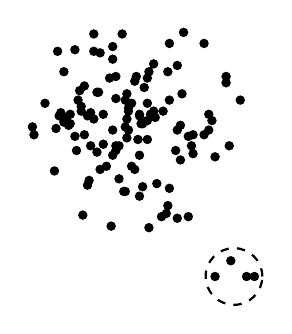
\begin{tikzpicture}[thick,scale=2, every node/.style={scale=5}]
			\fill (1.21, 0.56)  circle (0.3mm) (0.51, 1.02)  circle (0.3mm) (0.61, 1.44)  circle (0.3mm) (0.91, 1.54)  circle (0.3mm) (0.69, 0.58)  circle (0.3mm) (1.2, 1.3)  circle (0.3mm) (1.28, 0.96)  circle (0.3mm) (0.67, 1.21)  circle (0.3mm) (0.34, 0.95)  circle (0.3mm) (0.89, 0.83)  circle (0.3mm) (1.33, 0.38)  circle (0.3mm) (1.3, 1.55)  circle (0.3mm) (1.07, 0.99)  circle (0.3mm) (0.89, 0.62)  circle (0.3mm) (1.07, 0.87)  circle (0.3mm) (0.48, 0.67)  circle (0.3mm) (0.35, 0.9)  circle (0.3mm) (1.26, 1.34)  circle (0.3mm) (0.73, 1.54)  circle (0.3mm) (0.76, 1.17)  circle (0.3mm) (1.02, 1.03)  circle (0.3mm) (1.28, 0.74)  circle (0.3mm) (0.54, 1.3)  circle (0.3mm) (0.73, 1.43)  circle (0.3mm) (0.77, 1.42)  circle (0.3mm) (0.85, 0.93)  circle (0.3mm) (0.97, 1.1)  circle (0.3mm) (1.08, 1.3)  circle (0.3mm) (0.5, 1.43)  circle (0.3mm) (1.25, 0.8)  circle (0.3mm) (1.59, 0.83)  circle (0.3mm) (1.02, 0.51)  circle (0.3mm) (0.79, 0.84)  circle (0.3mm) (1.11, 1.05)  circle (0.3mm) (1.2, 0.45)  circle (0.3mm) (1.66, 1.12)  circle (0.3mm) (0.66, 0.39)  circle (0.3mm) (1.57, 1.27)  circle (0.3mm) (1.19, 0.4)  circle (0.3mm) (0.84, 0.32)  circle (0.3mm) (1.36, 0.9)  circle (0.3mm) (1.21, 1.48)  circle (0.3mm) (1.04, 0.57)  circle (0.3mm) (0.87, 0.83)  circle (0.3mm) (0.92, 0.54)  circle (0.3mm) (0.85, 1.46)  circle (0.3mm) (1.16, 0.38)  circle (0.3mm) (0.94, 0.88)  circle (0.3mm) (1.13, 0.59)  circle (0.3mm) (0.71, 0.83)  circle (0.3mm) (1.26, 0.37)  circle (0.3mm) (1.07, 0.87)  circle (0.3mm) (1.57, 1.23)  circle (0.3mm) (0.62, 0.8)  circle (0.3mm) (1.5, 0.76)  circle (0.3mm) (0.42, 1.1)  circle (0.3mm) (1.43, 1.48)  circle (0.3mm) (1.43, 0.9)  circle (0.3mm) (0.49, 0.94)  circle (0.3mm) (1.08, 0.31)  circle (0.3mm)

			(1.04, 0.97)  circle (0.3mm) (0.95, 0.93)  circle (0.3mm) (1.05, 1.2)  circle (0.3mm) (0.54, 0.98)  circle (0.3mm) (0.71, 1.04)  circle (0.3mm) (0.75, 1.17)  circle (0.3mm) (1.07, 1.26)  circle (0.3mm) (0.63, 1.12)  circle (0.3mm) (0.65, 1.08)  circle (0.3mm) (0.95, 1.05)  circle (0.3mm) (0.83, 1.26)  circle (0.3mm) (0.77, 0.68)  circle (0.3mm) (1.02, 0.77)  circle (0.3mm) (0.64, 1.18)  circle (0.3mm) (0.99, 0.68)  circle (0.3mm) (1.21, 1.12)  circle (0.3mm) (0.75, 0.79)  circle (0.3mm) (1.17, 1.05)  circle (0.3mm) (1.01, 0.87)  circle (0.3mm) (0.69, 1.02)  circle (0.3mm) (1.46, 0.93)  circle (0.3mm) (1.02, 1.02)  circle (0.3mm) (1.26, 0.93)  circle (0.3mm) (1.12, 1.01)  circle (0.3mm) (1.46, 1.03)  circle (0.3mm) (0.93, 0.95)  circle (0.3mm) (0.67, 0.9)  circle (0.3mm) (1.0, 1.27)  circle (0.3mm) (0.99, 1.24)  circle (0.3mm) (0.81, 0.7)  circle (0.3mm) (0.93, 0.54)  circle (0.3mm) (0.97, 0.7)  circle (0.3mm) (0.57, 0.96)  circle (0.3mm) (0.55, 1.01)  circle (0.3mm) (1.33, 0.89)  circle (0.3mm) (0.87, 0.8)  circle (0.3mm) (1.11, 1.35)  circle (0.3mm) (0.85, 1.38)  circle (0.3mm) (0.52, 1.04)  circle (0.3mm) (0.7, 0.61)  circle (0.3mm) (1.48, 0.99)  circle (0.3mm) (1.03, 0.97)  circle (0.3mm) (1.07, 1.1)  circle (0.3mm) (0.65, 1.05)  circle (0.3mm) (0.73, 1.0)  circle (0.3mm) (0.87, 1.13)  circle (0.3mm) (0.87, 1.27)  circle (0.3mm) (1.29, 1.16)  circle (0.3mm) (0.79, 1.03)  circle (0.3mm) (0.94, 1.0)  circle (0.3mm) (0.61, 0.89)  circle (0.3mm) (1.35, 0.83)  circle (0.3mm) (1.36, 0.78)  circle (0.3mm) (0.94, 1.16)  circle (0.3mm) (1.09, 1.03)  circle (0.3mm) (0.85, 0.77)  circle (0.3mm) (0.58, 1.03)  circle (0.3mm) (0.95, 1.07)  circle (0.3mm) (0.58, 0.97)  circle (0.3mm) (0.93, 1.12)  circle (0.3mm);
			\draw[dashed] (1.62,0) circle (1.8mm);
			\fill (1.7,0)  circle (0.3mm) (1.75,0)  circle (0.3mm) (1.5,0)  circle (0.3mm) (1.6,0.1)  circle (0.3mm);
		\end{tikzpicture}};
\end{frame}


\begin{frame}
	\frametitle{Types of Outliers (2)}
	\begin{itemize}
		\item \textbf{\color{airforceblue}Collective} \textbf{outlier}:
		      \begin{itemize}
			      \item A \textbf{subset} of data objects that collectively \\
			            deviates significantly from the whole data set.
			      \item Ex.: intrusion detection -- a number of computers \\
			            keep sending denial-of-service packages to each other.
		      \end{itemize}

		\item \textbf{Detection of collective outliers:}
		      \begin{itemize}
			      \item Consider not only behavior of individual objects,but also that of groups of objects.
			      \item Need to have the background knowledge on the relationship among data objects, such as a distance or similarity measure on objects.
		      \end{itemize}
		\item \textbf{A data set may have multiple types of outliers.}
		\item \textbf{One object may belong to more than one type of outlier.}
	\end{itemize}

	\tikzoverlay at (11cm,6cm) {
		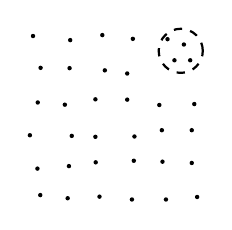
\begin{tikzpicture}[thick,scale=0.4, every node/.style={scale=5}]
			\fill (0.14, 0.02)  circle (0.7mm) (0.05, 0.86)  circle (0.7mm) (-0.19, 1.92)  circle (0.7mm) (0.06, 2.96)  circle (0.7mm) (0.15, 4.06)  circle (0.7mm) (-0.09, 5.07)  circle (0.7mm) (1.01, -0.08)  circle (0.7mm) (1.05, 0.94)  circle (0.7mm) (1.14, 1.9)  circle (0.7mm) (0.92, 2.89)  circle (0.7mm) (1.07, 4.05)  circle (0.7mm) (1.09, 4.94)  circle (0.7mm) (2.02, -0.03)  circle (0.7mm) (1.9, 1.06)  circle (0.7mm) (1.89, 1.87)  circle (0.7mm) (1.89, 3.06)  circle (0.7mm) (2.19, 3.98)  circle 	(0.7mm) (2.11, 5.1)  circle (0.7mm) (3.05, -0.12)  circle (0.7mm) (3.11, 1.11)  circle (0.7mm) (3.13, 1.88)  circle (0.7mm) (2.9, 3.05)  circle (0.7mm) (2.9, 3.88)  circle (0.7mm) (3.08, 4.98)  circle (0.7mm) (4.13, -0.12)  circle (0.7mm) (4.02, 1.08)  circle (0.7mm) (4.0, 2.08)  circle (0.7mm) (3.92, 2.88)  circle (0.7mm) (4.4, 4.3)  circle (0.7mm) (4.18, 4.97)  circle (0.7mm) (5.12, -0.04)  circle (0.7mm) (4.95, 1.04)  circle (0.7mm) (4.95, 2.08)  circle (0.7mm) (5.03, 2.91)  circle (0.7mm) (4.9, 4.3)  circle (0.7mm) (4.7, 4.8)  circle (0.7mm) ;
			\draw[dashed] (4.6,4.6) circle (7mm);
		\end{tikzpicture}};
\end{frame}


\begin{frame}{Challenges of Outlier Detection}
	\begin{itemize}
		\item \textbf{Modeling normal objects and outliers properly.}
		      \begin{itemize}
			      \item Hard to enumerate all possible normal behaviors in an application.
			      \item The border between normal and outlier objects is often a grey area.
		      \end{itemize}
		\item \textbf{Application-specific outlier detection.}
		      \begin{itemize}
			      \item Choice of distance measure among objects and the model of \\
			            relationship among objects are application-dependent.
			      \item E.g. clinical data: a small deviation could be an outlier; \\
			            while in marketing analysis: larger fluctuations.
		      \end{itemize}
	\end{itemize}
\end{frame}


\begin{frame}{Challenges of Outlier Detection (II)}
	\begin{itemize}
		\item \textbf{Handling noise in outlier detection.}
		      \begin{itemize}
			      \item Noise may distort the normal objects and blur the distinction \\
			            between normal objects and outliers.
			      \item It may hide outliers and reduce the effectiveness of outlier detection.
		      \end{itemize}
		\item \textbf{Understandability.}
		      \begin{itemize}
			      \item Understand why these are outliers: justification of the detection.
			      \item Specify the degree of an outlier: \\
			            the unlikelihood of the object being generated by a normal mechanism.
		      \end{itemize}
	\end{itemize}
\end{frame}

\section{Outlier-Detection Methods}

% TODO: make slide more rounded
\begin{frame}{How can we detect outliers?}
	\textbf{Two ways to categorize outlier-detection methods:}

	Grouping according to
	\begin{enumerate}
		\item \textcolor{faugray}{\textbf{How many samples are labeled:}}\\
		      I.e. supervised, semi-supervised vs. unsupervised methods.
		\item \textcolor{faugray}{\textbf{Assumptions}} regarding normal and abnormal samples.\\
		      I.e. statistical, proximity-based, and clustering-based methods.
	\end{enumerate}
\end{frame}


\begin{frame}{Outlier Detection: Grouping According to Label Existence I}
	Domain expert labelled all, some, or no samples.
	\vspace*{1em}
	\textcolor{faugray}{\textbf{Supervised Methods:}}
	\begin{itemize}
		\item Modeling outlier detection as a \textbf{classification problem}:\\
		      Samples examined by domain experts used for training \& testing.
		\item Methods for learning a classifier for outlier detection effectively:
		      \begin{itemize}
			      \item Model normal objects \& report those not matching the model as outliers.
			      \item Model outliers and treat those not matching the model as normal.
		      \end{itemize}
		\item \textbf{Challenges:}
		      \begin{itemize}
			      \item Imbalanced classes, i.e., outliers are rare: \\
			            Boost the outlier class and make up some artificial outliers.
			      \item Catch as many outliers as possible. \\
			            Therefore: recall is more important than accuracy \\
			            (i.e., not mislabeling normal objects as outliers).
		      \end{itemize}
	\end{itemize}
\end{frame}


\begin{frame}{Outlier Detection: Grouping According to Label Existence II}
	\textcolor{faugray}{\textbf{Unsupervised Methods:}}

	\begin{itemize}
		\item No labels available.
		\item \textbf{Implicit assumptions:}
		      \begin{itemize}
			      \item \textcolor{faugray}{Normal objects are somewhat ``clustered''} into multiple groups, each having some distinct features.
			      \item Outlier are expected to be far away from any group of normal objects.
		      \end{itemize}
		\item Adapt clustering methods for unsupervised outlier detection:
		      \begin{enumerate}
			      \item Find clusters.
			      \item Samples not falling in any cluster are outliers.
		      \end{enumerate}
		\item \textbf{Challenges:}
		      \begin{itemize}
			      \item Samples outside of clusters may not be outliers.
			      \item Costly to find clusters.
			      \item Hard to distinguish noise from outliers.
			      \item Can't detect collective outliers effectively.
		      \end{itemize}
	\end{itemize}
\end{frame}


\begin{frame}
	\frametitle{Outlier Detection: Grouping According to Label Existence III}
	\textcolor{faugray}{\textbf{Semi-Supervised Methods:}}
	\begin{itemize}
		\item Only a small set of samples are labeled as normal or as outlier.
		\item \textbf{If some {\color{airforceblue}labeled normal objects} are available:}
		      \begin{itemize}
			      \item Use the labeled examples and the proximate \\
			            unlabeled objects to train a model for normal objects.
			      \item Those not fitting the model of normal objects are detected as outliers.
		      \end{itemize}
		\item \textbf{If only some {\color{airforceblue}labeled outliers} are available, \\ that small number may not cover all possible outliers well.}
		      \begin{itemize}
			      \item To improve the quality of outlier detection: get help from models for normal objects learned from unsupervised methods.
		      \end{itemize}
	\end{itemize}
\end{frame}


\begin{frame}{Outlier Detection: Grouping Based on Assumption I}
	\tikzoverlay at (11cm,1cm) {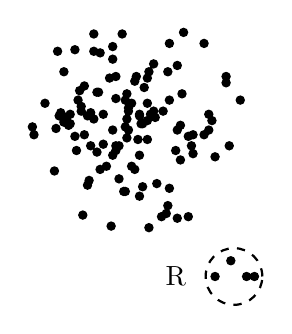
\begin{tikzpicture}[thick,scale=2, every node/.style={scale=5}]
	\fill (1.21, 0.56)  circle (0.3mm) (0.51, 1.02)  circle (0.3mm) (0.61, 1.44)  circle (0.3mm) (0.91, 1.54)  circle (0.3mm) (0.69, 0.58)  circle (0.3mm) (1.2, 1.3)  circle (0.3mm) (1.28, 0.96)  circle (0.3mm) (0.67, 1.21)  circle (0.3mm) (0.34, 0.95)  circle (0.3mm) (0.89, 0.83)  circle (0.3mm) (1.33, 0.38)  circle (0.3mm) (1.3, 1.55)  circle (0.3mm) (1.07, 0.99)  circle (0.3mm) (0.89, 0.62)  circle (0.3mm) (1.07, 0.87)  circle (0.3mm) (0.48, 0.67)  circle (0.3mm) (0.35, 0.9)  circle (0.3mm) (1.26, 1.34)  circle (0.3mm) (0.73, 1.54)  circle (0.3mm) (0.76, 1.17)  circle (0.3mm) (1.02, 1.03)  circle (0.3mm) (1.28, 0.74)  circle (0.3mm) (0.54, 1.3)  circle (0.3mm) (0.73, 1.43)  circle (0.3mm) (0.77, 1.42)  circle (0.3mm) (0.85, 0.93)  circle (0.3mm) (0.97, 1.1)  circle (0.3mm) (1.08, 1.3)  circle (0.3mm) (0.5, 1.43)  circle (0.3mm) (1.25, 0.8)  circle (0.3mm) (1.59, 0.83)  circle (0.3mm) (1.02, 0.51)  circle (0.3mm) (0.79, 0.84)  circle (0.3mm) (1.11, 1.05)  circle (0.3mm) (1.2, 0.45)  circle (0.3mm) (1.66, 1.12)  circle (0.3mm) (0.66, 0.39)  circle (0.3mm) (1.57, 1.27)  circle (0.3mm) (1.19, 0.4)  circle (0.3mm) (0.84, 0.32)  circle (0.3mm) (1.36, 0.9)  circle (0.3mm) (1.21, 1.48)  circle (0.3mm) (1.04, 0.57)  circle (0.3mm) (0.87, 0.83)  circle (0.3mm) (0.92, 0.54)  circle (0.3mm) (0.85, 1.46)  circle (0.3mm) (1.16, 0.38)  circle (0.3mm) (0.94, 0.88)  circle (0.3mm) (1.13, 0.59)  circle (0.3mm) (0.71, 0.83)  circle (0.3mm) (1.26, 0.37)  circle (0.3mm) (1.07, 0.87)  circle (0.3mm) (1.57, 1.23)  circle (0.3mm) (0.62, 0.8)  circle (0.3mm) (1.5, 0.76)  circle (0.3mm) (0.42, 1.1)  circle (0.3mm) (1.43, 1.48)  circle (0.3mm) (1.43, 0.9)  circle (0.3mm) (0.49, 0.94)  circle (0.3mm) (1.08, 0.31)  circle (0.3mm)

	(1.04, 0.97)  circle (0.3mm) (0.95, 0.93)  circle (0.3mm) (1.05, 1.2)  circle (0.3mm) (0.54, 0.98)  circle (0.3mm) (0.71, 1.04)  circle (0.3mm) (0.75, 1.17)  circle (0.3mm) (1.07, 1.26)  circle (0.3mm) (0.63, 1.12)  circle (0.3mm) (0.65, 1.08)  circle (0.3mm) (0.95, 1.05)  circle (0.3mm) (0.83, 1.26)  circle (0.3mm) (0.77, 0.68)  circle (0.3mm) (1.02, 0.77)  circle (0.3mm) (0.64, 1.18)  circle (0.3mm) (0.99, 0.68)  circle (0.3mm) (1.21, 1.12)  circle (0.3mm) (0.75, 0.79)  circle (0.3mm) (1.17, 1.05)  circle (0.3mm) (1.01, 0.87)  circle (0.3mm) (0.69, 1.02)  circle (0.3mm) (1.46, 0.93)  circle (0.3mm) (1.02, 1.02)  circle (0.3mm) (1.26, 0.93)  circle (0.3mm) (1.12, 1.01)  circle (0.3mm) (1.46, 1.03)  circle (0.3mm) (0.93, 0.95)  circle (0.3mm) (0.67, 0.9)  circle (0.3mm) (1.0, 1.27)  circle (0.3mm) (0.99, 1.24)  circle (0.3mm) (0.81, 0.7)  circle (0.3mm) (0.93, 0.54)  circle (0.3mm) (0.97, 0.7)  circle (0.3mm) (0.57, 0.96)  circle (0.3mm) (0.55, 1.01)  circle (0.3mm) (1.33, 0.89)  circle (0.3mm) (0.87, 0.8)  circle (0.3mm) (1.11, 1.35)  circle (0.3mm) (0.85, 1.38)  circle (0.3mm) (0.52, 1.04)  circle (0.3mm) (0.7, 0.61)  circle (0.3mm) (1.48, 0.99)  circle (0.3mm) (1.03, 0.97)  circle (0.3mm) (1.07, 1.1)  circle (0.3mm) (0.65, 1.05)  circle (0.3mm) (0.73, 1.0)  circle (0.3mm) (0.87, 1.13)  circle (0.3mm) (0.87, 1.27)  circle (0.3mm) (1.29, 1.16)  circle (0.3mm) (0.79, 1.03)  circle (0.3mm) (0.94, 1.0)  circle (0.3mm) (0.61, 0.89)  circle (0.3mm) (1.35, 0.83)  circle (0.3mm) (1.36, 0.78)  circle (0.3mm) (0.94, 1.16)  circle (0.3mm) (1.09, 1.03)  circle (0.3mm) (0.85, 0.77)  circle (0.3mm) (0.58, 1.03)  circle (0.3mm) (0.95, 1.07)  circle (0.3mm) (0.58, 0.97)  circle (0.3mm) (0.93, 1.12)  circle (0.3mm);

	\draw[dashed] (1.62,0) circle (1.8mm);
	\fill (1.7,0)  circle (0.3mm) (1.75,0)  circle (0.3mm) (1.5,0)  circle (0.3mm) (1.6,0.1)  circle (0.3mm);
	\node[scale = 0.2] at (1.25,0)    {R};

\end{tikzpicture}
};
	\textcolor{faugray}{\textbf{Statistical Methods}}
	\begin{itemize}
		\item (Also known as model-based methods)
		\item Assume that the \textbf{\color{airforceblue}normal data follow some statistical model}.
		      \begin{itemize}
			      \item The data not following the model are outliers.
		      \end{itemize}
		\item \textbf{Example (right figure):}
		      \begin{itemize}
			      \item First use Gaussian distribution $\mathcal{N}_D(x \; \vert \; \mu,\sigma)$ to model the normal data.
			      \item For each object $y$ in region $R$, estimate $\mathcal{N}_D(y \; \vert \; \mu, \sigma)$, the probability that $y$ \\
			            fits the Gaussian distribution.
			      \item If $\mathcal{N}_D(y \; \vert \; \mu, \sigma)$ is very low, $y$ is unlikely generated by the Gaussian model, thus an outlier.
		      \end{itemize}
		      \item\textbf{Effectiveness of statistical methods:}
		      \begin{itemize}
			      \item Highly depends on whether the assumption of statistical model holds in the real data.
		      \end{itemize}
		\item \textbf{There are many kinds of statistical models.}
		      \begin{itemize}
			      \item E.g., parametric vs. non-parametric.
		      \end{itemize}
	\end{itemize}
\end{frame}


\begin{frame}{Outlier Detection: Grouping Based on Assumption II}
	\tikzoverlay at (11cm,1cm) {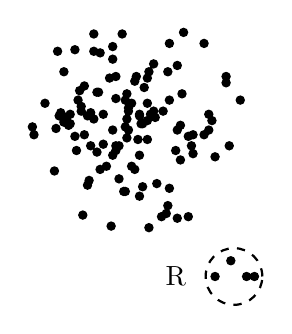
\begin{tikzpicture}[thick,scale=2, every node/.style={scale=5}]
	\fill (1.21, 0.56)  circle (0.3mm) (0.51, 1.02)  circle (0.3mm) (0.61, 1.44)  circle (0.3mm) (0.91, 1.54)  circle (0.3mm) (0.69, 0.58)  circle (0.3mm) (1.2, 1.3)  circle (0.3mm) (1.28, 0.96)  circle (0.3mm) (0.67, 1.21)  circle (0.3mm) (0.34, 0.95)  circle (0.3mm) (0.89, 0.83)  circle (0.3mm) (1.33, 0.38)  circle (0.3mm) (1.3, 1.55)  circle (0.3mm) (1.07, 0.99)  circle (0.3mm) (0.89, 0.62)  circle (0.3mm) (1.07, 0.87)  circle (0.3mm) (0.48, 0.67)  circle (0.3mm) (0.35, 0.9)  circle (0.3mm) (1.26, 1.34)  circle (0.3mm) (0.73, 1.54)  circle (0.3mm) (0.76, 1.17)  circle (0.3mm) (1.02, 1.03)  circle (0.3mm) (1.28, 0.74)  circle (0.3mm) (0.54, 1.3)  circle (0.3mm) (0.73, 1.43)  circle (0.3mm) (0.77, 1.42)  circle (0.3mm) (0.85, 0.93)  circle (0.3mm) (0.97, 1.1)  circle (0.3mm) (1.08, 1.3)  circle (0.3mm) (0.5, 1.43)  circle (0.3mm) (1.25, 0.8)  circle (0.3mm) (1.59, 0.83)  circle (0.3mm) (1.02, 0.51)  circle (0.3mm) (0.79, 0.84)  circle (0.3mm) (1.11, 1.05)  circle (0.3mm) (1.2, 0.45)  circle (0.3mm) (1.66, 1.12)  circle (0.3mm) (0.66, 0.39)  circle (0.3mm) (1.57, 1.27)  circle (0.3mm) (1.19, 0.4)  circle (0.3mm) (0.84, 0.32)  circle (0.3mm) (1.36, 0.9)  circle (0.3mm) (1.21, 1.48)  circle (0.3mm) (1.04, 0.57)  circle (0.3mm) (0.87, 0.83)  circle (0.3mm) (0.92, 0.54)  circle (0.3mm) (0.85, 1.46)  circle (0.3mm) (1.16, 0.38)  circle (0.3mm) (0.94, 0.88)  circle (0.3mm) (1.13, 0.59)  circle (0.3mm) (0.71, 0.83)  circle (0.3mm) (1.26, 0.37)  circle (0.3mm) (1.07, 0.87)  circle (0.3mm) (1.57, 1.23)  circle (0.3mm) (0.62, 0.8)  circle (0.3mm) (1.5, 0.76)  circle (0.3mm) (0.42, 1.1)  circle (0.3mm) (1.43, 1.48)  circle (0.3mm) (1.43, 0.9)  circle (0.3mm) (0.49, 0.94)  circle (0.3mm) (1.08, 0.31)  circle (0.3mm)

	(1.04, 0.97)  circle (0.3mm) (0.95, 0.93)  circle (0.3mm) (1.05, 1.2)  circle (0.3mm) (0.54, 0.98)  circle (0.3mm) (0.71, 1.04)  circle (0.3mm) (0.75, 1.17)  circle (0.3mm) (1.07, 1.26)  circle (0.3mm) (0.63, 1.12)  circle (0.3mm) (0.65, 1.08)  circle (0.3mm) (0.95, 1.05)  circle (0.3mm) (0.83, 1.26)  circle (0.3mm) (0.77, 0.68)  circle (0.3mm) (1.02, 0.77)  circle (0.3mm) (0.64, 1.18)  circle (0.3mm) (0.99, 0.68)  circle (0.3mm) (1.21, 1.12)  circle (0.3mm) (0.75, 0.79)  circle (0.3mm) (1.17, 1.05)  circle (0.3mm) (1.01, 0.87)  circle (0.3mm) (0.69, 1.02)  circle (0.3mm) (1.46, 0.93)  circle (0.3mm) (1.02, 1.02)  circle (0.3mm) (1.26, 0.93)  circle (0.3mm) (1.12, 1.01)  circle (0.3mm) (1.46, 1.03)  circle (0.3mm) (0.93, 0.95)  circle (0.3mm) (0.67, 0.9)  circle (0.3mm) (1.0, 1.27)  circle (0.3mm) (0.99, 1.24)  circle (0.3mm) (0.81, 0.7)  circle (0.3mm) (0.93, 0.54)  circle (0.3mm) (0.97, 0.7)  circle (0.3mm) (0.57, 0.96)  circle (0.3mm) (0.55, 1.01)  circle (0.3mm) (1.33, 0.89)  circle (0.3mm) (0.87, 0.8)  circle (0.3mm) (1.11, 1.35)  circle (0.3mm) (0.85, 1.38)  circle (0.3mm) (0.52, 1.04)  circle (0.3mm) (0.7, 0.61)  circle (0.3mm) (1.48, 0.99)  circle (0.3mm) (1.03, 0.97)  circle (0.3mm) (1.07, 1.1)  circle (0.3mm) (0.65, 1.05)  circle (0.3mm) (0.73, 1.0)  circle (0.3mm) (0.87, 1.13)  circle (0.3mm) (0.87, 1.27)  circle (0.3mm) (1.29, 1.16)  circle (0.3mm) (0.79, 1.03)  circle (0.3mm) (0.94, 1.0)  circle (0.3mm) (0.61, 0.89)  circle (0.3mm) (1.35, 0.83)  circle (0.3mm) (1.36, 0.78)  circle (0.3mm) (0.94, 1.16)  circle (0.3mm) (1.09, 1.03)  circle (0.3mm) (0.85, 0.77)  circle (0.3mm) (0.58, 1.03)  circle (0.3mm) (0.95, 1.07)  circle (0.3mm) (0.58, 0.97)  circle (0.3mm) (0.93, 1.12)  circle (0.3mm);

	\draw[dashed] (1.62,0) circle (1.8mm);
	\fill (1.7,0)  circle (0.3mm) (1.75,0)  circle (0.3mm) (1.5,0)  circle (0.3mm) (1.6,0.1)  circle (0.3mm);
	\node[scale = 0.2] at (1.25,0)    {R};

\end{tikzpicture}
};
	\textcolor{faugray}{\textbf{Proximity-Based Methods}}

	An object is an outlier if the \textbf{\color{airforceblue}nearest neighbors of the object are far away},\\ i.e., the proximity of the object significantly deviates from the proximity\\ of most of the other objects in the same data set.
	\begin{itemize}

		\item \textbf{Example (right figure):}
		      \begin{itemize}
			      \item Model the proximity of an object using its 3 nearest neighbors.
			      \item Objects in region R are substantially different from other objects in the data set.
			      \item Thus the objects in R are outliers.
		      \end{itemize}
		\item \textbf{Effectiveness of proximity-based methods:}
		      \begin{itemize}
			      \item Highly relies on the proximity measure.
			      \item In some applications, proximity or distance measures cannot be obtained easily.
			      \item Often have a difficulty in finding a group of outliers which are close to each other.
		      \end{itemize}
		\item \textbf{Two major types of proximity-based outlier detection:}
		      \begin{itemize}
			      \item Distance-based vs. density-based.
		      \end{itemize}
	\end{itemize}
\end{frame}


\begin{frame}{Outlier Detection: Grouping Based on Assumption III}
	\tikzoverlay at (11cm,1cm) {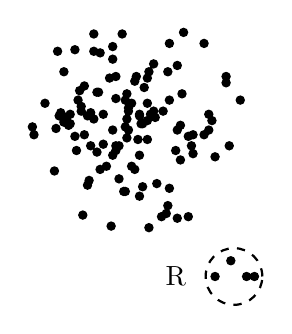
\begin{tikzpicture}[thick,scale=2, every node/.style={scale=5}]
	\fill (1.21, 0.56)  circle (0.3mm) (0.51, 1.02)  circle (0.3mm) (0.61, 1.44)  circle (0.3mm) (0.91, 1.54)  circle (0.3mm) (0.69, 0.58)  circle (0.3mm) (1.2, 1.3)  circle (0.3mm) (1.28, 0.96)  circle (0.3mm) (0.67, 1.21)  circle (0.3mm) (0.34, 0.95)  circle (0.3mm) (0.89, 0.83)  circle (0.3mm) (1.33, 0.38)  circle (0.3mm) (1.3, 1.55)  circle (0.3mm) (1.07, 0.99)  circle (0.3mm) (0.89, 0.62)  circle (0.3mm) (1.07, 0.87)  circle (0.3mm) (0.48, 0.67)  circle (0.3mm) (0.35, 0.9)  circle (0.3mm) (1.26, 1.34)  circle (0.3mm) (0.73, 1.54)  circle (0.3mm) (0.76, 1.17)  circle (0.3mm) (1.02, 1.03)  circle (0.3mm) (1.28, 0.74)  circle (0.3mm) (0.54, 1.3)  circle (0.3mm) (0.73, 1.43)  circle (0.3mm) (0.77, 1.42)  circle (0.3mm) (0.85, 0.93)  circle (0.3mm) (0.97, 1.1)  circle (0.3mm) (1.08, 1.3)  circle (0.3mm) (0.5, 1.43)  circle (0.3mm) (1.25, 0.8)  circle (0.3mm) (1.59, 0.83)  circle (0.3mm) (1.02, 0.51)  circle (0.3mm) (0.79, 0.84)  circle (0.3mm) (1.11, 1.05)  circle (0.3mm) (1.2, 0.45)  circle (0.3mm) (1.66, 1.12)  circle (0.3mm) (0.66, 0.39)  circle (0.3mm) (1.57, 1.27)  circle (0.3mm) (1.19, 0.4)  circle (0.3mm) (0.84, 0.32)  circle (0.3mm) (1.36, 0.9)  circle (0.3mm) (1.21, 1.48)  circle (0.3mm) (1.04, 0.57)  circle (0.3mm) (0.87, 0.83)  circle (0.3mm) (0.92, 0.54)  circle (0.3mm) (0.85, 1.46)  circle (0.3mm) (1.16, 0.38)  circle (0.3mm) (0.94, 0.88)  circle (0.3mm) (1.13, 0.59)  circle (0.3mm) (0.71, 0.83)  circle (0.3mm) (1.26, 0.37)  circle (0.3mm) (1.07, 0.87)  circle (0.3mm) (1.57, 1.23)  circle (0.3mm) (0.62, 0.8)  circle (0.3mm) (1.5, 0.76)  circle (0.3mm) (0.42, 1.1)  circle (0.3mm) (1.43, 1.48)  circle (0.3mm) (1.43, 0.9)  circle (0.3mm) (0.49, 0.94)  circle (0.3mm) (1.08, 0.31)  circle (0.3mm)

	(1.04, 0.97)  circle (0.3mm) (0.95, 0.93)  circle (0.3mm) (1.05, 1.2)  circle (0.3mm) (0.54, 0.98)  circle (0.3mm) (0.71, 1.04)  circle (0.3mm) (0.75, 1.17)  circle (0.3mm) (1.07, 1.26)  circle (0.3mm) (0.63, 1.12)  circle (0.3mm) (0.65, 1.08)  circle (0.3mm) (0.95, 1.05)  circle (0.3mm) (0.83, 1.26)  circle (0.3mm) (0.77, 0.68)  circle (0.3mm) (1.02, 0.77)  circle (0.3mm) (0.64, 1.18)  circle (0.3mm) (0.99, 0.68)  circle (0.3mm) (1.21, 1.12)  circle (0.3mm) (0.75, 0.79)  circle (0.3mm) (1.17, 1.05)  circle (0.3mm) (1.01, 0.87)  circle (0.3mm) (0.69, 1.02)  circle (0.3mm) (1.46, 0.93)  circle (0.3mm) (1.02, 1.02)  circle (0.3mm) (1.26, 0.93)  circle (0.3mm) (1.12, 1.01)  circle (0.3mm) (1.46, 1.03)  circle (0.3mm) (0.93, 0.95)  circle (0.3mm) (0.67, 0.9)  circle (0.3mm) (1.0, 1.27)  circle (0.3mm) (0.99, 1.24)  circle (0.3mm) (0.81, 0.7)  circle (0.3mm) (0.93, 0.54)  circle (0.3mm) (0.97, 0.7)  circle (0.3mm) (0.57, 0.96)  circle (0.3mm) (0.55, 1.01)  circle (0.3mm) (1.33, 0.89)  circle (0.3mm) (0.87, 0.8)  circle (0.3mm) (1.11, 1.35)  circle (0.3mm) (0.85, 1.38)  circle (0.3mm) (0.52, 1.04)  circle (0.3mm) (0.7, 0.61)  circle (0.3mm) (1.48, 0.99)  circle (0.3mm) (1.03, 0.97)  circle (0.3mm) (1.07, 1.1)  circle (0.3mm) (0.65, 1.05)  circle (0.3mm) (0.73, 1.0)  circle (0.3mm) (0.87, 1.13)  circle (0.3mm) (0.87, 1.27)  circle (0.3mm) (1.29, 1.16)  circle (0.3mm) (0.79, 1.03)  circle (0.3mm) (0.94, 1.0)  circle (0.3mm) (0.61, 0.89)  circle (0.3mm) (1.35, 0.83)  circle (0.3mm) (1.36, 0.78)  circle (0.3mm) (0.94, 1.16)  circle (0.3mm) (1.09, 1.03)  circle (0.3mm) (0.85, 0.77)  circle (0.3mm) (0.58, 1.03)  circle (0.3mm) (0.95, 1.07)  circle (0.3mm) (0.58, 0.97)  circle (0.3mm) (0.93, 1.12)  circle (0.3mm);

	\draw[dashed] (1.62,0) circle (1.8mm);
	\fill (1.7,0)  circle (0.3mm) (1.75,0)  circle (0.3mm) (1.5,0)  circle (0.3mm) (1.6,0.1)  circle (0.3mm);
	\node[scale = 0.2] at (1.25,0)    {R};

\end{tikzpicture}
};
	\textcolor{faugray}{\textbf{Clustering-Based Methods}}

	Normal data belong to large and dense clusters, whereas outliers belong to\\ \textbf{\color{airforceblue}small or sparse clusters}, or do not belong to any cluster.
	\begin{itemize}

		\item \textbf{Example (right figure): Two clusters.}
		      \begin{itemize}
			      \item All points not in R form a large cluster.
			      \item The two points in R form a tiny cluster, thus are outliers.

		      \end{itemize}
		\item \textbf{Many clustering methods:}
		      \begin{itemize}
			      \item Thus also many clustering-based outlier detection methods.
		      \end{itemize}
		\item \textbf{Clustering is expensive.}
		      \begin{itemize}
			      \item Straightforward adaptation of a clustering method for outlier detection can be costly and does not scale up well for large data sets.
		      \end{itemize}
	\end{itemize}
\end{frame}

\section{Statistical Approaches}


\begin{frame}
	\frametitle{Statistical Approaches}
	Assume that the objects in a data set are \textbf{\color{airforceblue}generated by a stochastic process} (a generative model).
	\begin{itemize}
		\item \textbf{Idea:}
		      \begin{itemize}
			      \item Learn a generative model fitting the given data set, and then identify the objects in low-probability regions of the model as outliers.
		      \end{itemize}
		\item \textbf{Methods divided into two categories:}
		      \begin{itemize}
			      \item Parametric vs. non-parametric.
		      \end{itemize}
		\item \textbf{Parametric method}
		      \begin{itemize}
			      \item Assumes that the normal data is generated \\
			            by a parametric distribution with parameter $\theta$.
			      \item The probability density function of the parametric distribution $f(x, \theta)$ \\
			            gives the probability that object $x$ is generated by the distribution.
			      \item The smaller this value, the more likely $x$ is an outlier.
		      \end{itemize}
	\end{itemize}
\end{frame}


\begin{frame}
	\frametitle{Statistical Approaches (2)}
	\begin{itemize}
		\item \textbf{Non-parametric method:}
		      \begin{itemize}
			      \item Do not assume an a-priori statistical model \\
			            and determine the model from the input data.
			      \item Not completely parameter-free, \\
			            but consider number and nature of the parameters to be flexible and \\ not fixed in advance.
			      \item \textbf{Examples:} \textbf{\color{airforceblue}histogram} and kernel-density estimation.
		      \end{itemize}
	\end{itemize}
\end{frame}


\begin{frame}
	\frametitle{Parametric Methods I: \\ Detection of Univariate Outliers Based on Normal Distribution}
	\begin{itemize}
		\item Univariate data:
		      \begin{itemize}
			      \item A data set involving only one attribute or variable.
		      \end{itemize}
		\item Assumption:
		      \begin{itemize}
			      \item Data are generated from a normal distribution.
		      \end{itemize}
		\item Learn the parameters from the input data, and identify the points with low probability as outliers.
		      \begin{itemize}
			      \item Use the \textbf{\color{airforceblue}maximum-likelihood method} to estimate $\mu$ and $\sigma$.
		      \end{itemize}
	\end{itemize}
\end{frame}


\begin{frame}
	\frametitle{The Maximum Likelihood Estimate of $\mu$}
	\begin{itemize}
		\item \textbf{Assumption:}
		      \begin{itemize}
			      \item Data is generated by an underlying Gaussian process. \\
			            Thus, the likelihood function $\mathcal{L}$ is the Gaussian process itself:
			            \begin{align}
				            \mathcal{L}(\mathbf{X}) = \text{P}(\mathbf{X} \; \vert \; \theta) = \mathcal{N}(\mathbf{X} \; \vert \; \theta) = \mathcal{N}(\mathbf{X} \; \vert \; \mu, \sigma).
			            \end{align}
		      \end{itemize}
		\item We need to find good estimates for $\mu$ and $\sigma$:
		      \begin{align}
			      \mu_{\text{MLE}} = \text{argmax}_{\mu} \; \mathcal{N}(\mathbf{X} \; \vert \; \mu, \sigma), \\
			      \sigma_{\text{MLE}} = \text{argmax}_{\sigma} \; \mathcal{N}(\mathbf{X} \; \vert \; \mu, \sigma).
		      \end{align}
		\item To make computation easier, as the product of probabilities $\prod$ turns into sums $\sum$ under the $\log$-function, we apply the logarithm. As $\log$ is monotonically increasing it holds that $\text{argmax}_{\theta} \; \log f(\theta) = \text{argmax}_{\theta} \; f(\theta)$.
	\end{itemize}
\end{frame}


\begin{frame}
	\frametitle{The Maximum Likelihood Estimate of $\mu$}
	\begin{itemize}
		\item We seek for the best parameters $\theta = \{\mu, \sigma\}$ for some dataset $\mathbf{X} = \{\mathbf{x}_1,\ldots,\mathbf{x}_n\}$ of $n$ data points. Thus we take the sum of the respective logarithms applied to the Gaussian:
		      \begin{align}
			      \log\left(\mathcal{N}(\mathbf{X} \; \vert \; \theta)\right) = \sum_{i=1}^{n} \log\left( \mathcal{N}(\mathbf{x}_i \; \vert \; \theta)\right) = \sum_{i=1}^{n} \log\left( \mathcal{N}(\mathbf{x}_i \; \vert \; \mu, \sigma)\right).
		      \end{align}
		\item The log-likelihood function then reads as:
		      \begin{align}
			      \sum_{i=1}^{n} \log\left(\mathcal{N}(\mathbf{x}_i \; \vert \; \mu, \sigma)\right) = \sum_{i=1}^{n} \log\left(\frac{1}{\sqrt{2\pi\sigma^2}} \cdot \exp \left( -\frac{1}{2} \left( \frac{(\mathbf{x_i}-\mu)^2}{\sigma^2} \right) \right)\right).
		      \end{align}
		\item Note, that we took a simplification here. The full covariance matrix $\Sigma$ is replaced keeping only the diagonal elements $\sigma^2$, which is the variance. This is known as the assumption of diagonal covariance matrices.
	\end{itemize}
\end{frame}


\begin{frame}
	\frametitle{The Maximum Likelihood Estimate of $\mu$}
	\begin{itemize}
		\item Next, we use some algebra to get the log-likelihood, denoted by $\log \mathcal{L}(\mathbf{X})$, into a nicer form:
		      \begin{align}
			      \log\left(\mathcal{L}(\mathbf{X})\right) & = \sum_{i=1}^{n} \log\left(\frac{1}{\sqrt{2\pi\sigma^2}} \cdot \exp\left( -\frac{1}{2} \left( \frac{(\mathbf{x}_i-\mu)^2}{\sigma^2} \right)\right)\right)              \\
			                                               & = \sum_{i=1}^{n} \log\left(\frac{1}{\sqrt{2\pi\sigma^2}}\right) + \log\left(\exp\left( -\frac{1}{2} \left( \frac{(\mathbf{x}_i-\mu)^2}{\sigma^2} \right)\right)\right) \\
			                                               & = \sum_{i=1}^{n} \log(1) - \log(\sqrt{2\pi\sigma^2}) + \log\left(\exp\left( -\frac{1}{2} \left( \frac{(\mathbf{x}_i-\mu)^2}{\sigma^2} \right)\right)\right)            \\
			                                               & = \sum_{i=1}^{n} \log(1) - \log\left(\sqrt{2\pi\sigma^2}\right) - \frac{1}{2} \left( \frac{(\mathbf{x}_i-\mu)^2}{\sigma^2} \right) \cdot \log(e).
		      \end{align}
		\item We simplify the computation taking $\log$ with base $e$. Thus $\log_e e = 1$. \\
		      It also applies, regardless of base, that $\log(1) = 0$.
	\end{itemize}
\end{frame}


\begin{frame}
	\frametitle{The Maximum Likelihood Estimate of $\mu$}
	\begin{itemize}
		\item Applying the logarithm with base $e$ yields:
		      \begin{align}
			      \log\left(\mathcal{L}(\mathbf{X})\right) & = \sum_{i=1}^{n} - \log\left(\sqrt{2\pi\sigma^2}\right) -\frac{1}{2} \left( \frac{(\mathbf{x}_i-\mu)^2}{\sigma^2} \right)        \\
			                                               & = \sum_{i=1}^{n} - \frac{1}{2} \log\left(2\pi\sigma^2\right) -\frac{1}{2} \left( \frac{(\mathbf{x}_i-\mu)^2}{\sigma^2} \right)   \\
			                                               & = - \frac{n}{2} \log\left(2\pi\sigma^2\right) + \sum_{i=1}^{n} -\frac{1}{2} \left( \frac{(\mathbf{x}_i-\mu)^2}{\sigma^2} \right) \\
			                                               & = - \frac{n}{2} \log\left(2\pi\sigma^2\right) - \frac{1}{2\sigma^2} \sum_{i=1}^{n} (\mathbf{x}_i-\mu)^2.
		      \end{align}
	\end{itemize}
\end{frame}


\begin{frame}
	\frametitle{The Maximum Likelihood Estimate of $\mu$}
	\begin{itemize}
		\item In order to get $\text{argmax}_\mu \log\left(\mathcal{L}(\mathbf{X})\right)$ we have to do two things:
		      \begin{itemize}
			      \item[1.] Derive the partial derivative of the function with respect to the parameter.
			      \item[2.] Set the partial derivative to zero, and solve for $\mu$.
		      \end{itemize}
		\item In the same way we get $\text{argmax}_\sigma \; \log\left(\mathcal{L}(\mathbf{X})\right)$. Thus,
		      \begin{align}
			      \text{argmax}_\mu \; \log\left(\mathcal{L}(\mathbf{X})\right) := \frac{\partial \log\left(\mathcal{L}(\mathbf{X})\right)}{\partial \mu} = 0.
		      \end{align}
		\item We need to find the following partial derivative:
		      \begin{align}
			      \frac{\partial \log\left(\mathcal{L}(\mathbf{X})\right)}{\partial \mu} = \frac{\partial}{\partial\mu} \left( - \frac{n}{2} \log\left(2\pi\sigma^2\right) -\frac{1}{2\sigma^2} \sum_{i=1}^{n} (\mathbf{x}_i-\mu)^2 \right).
		      \end{align}
	\end{itemize}
\end{frame}


\begin{frame}
	\frametitle{The Maximum Likelihood Estimate of $\mu$}
	\begin{itemize}
		\item We start to simplify our partial derivative:
		      \begin{align}
			      \frac{\partial \log\left(\mathcal{L}(\mathbf{X})\right)}{\partial \mu} & = \frac{\partial}{\partial\mu} \left( - \frac{n}{2} \log\left(2\pi\sigma^2\right) -\frac{1}{2\sigma^2} \sum_{i=1}^{n} (\mathbf{x}_i-\mu)^2 \right)                                            \\
			                                                                             & = \frac{\partial}{\partial\mu} \left( - \frac{n}{2} \log\left(2\pi\sigma^2\right)\right) + \frac{\partial}{\partial\mu}\left(-\frac{1}{2\sigma^2} \sum_{i=1}^{n} (\mathbf{x}_i-\mu)^2 \right) \\
			                                                                             & = 0 + \frac{\partial}{\partial\mu}\left(-\frac{1}{2\sigma^2} \sum_{i=1}^{n} (\mathbf{x}_i-\mu)^2 \right)                                                                                      \\
			                                                                             & = \frac{\partial}{\partial\mu}\left(-\frac{1}{2\sigma^2} \sum_{i=1}^{n} (\mathbf{x}_i-\mu)^2 \right).
		      \end{align}
	\end{itemize}
\end{frame}


\begin{frame}
	\frametitle{The Maximum Likelihood Estimate of $\mu$}
	\begin{itemize}
		\item Next, we move the partial operator inside the sum:
		      \begin{align}
			      \frac{\partial \log\left(\mathcal{L}(\mathbf{X})\right)}{\partial \mu} & = \frac{\partial}{\partial\mu}\left(-\frac{1}{2\sigma^2} \sum_{i=1}^{n} (\mathbf{x}_i-\mu)^2 \right)                                                                                                                     \\
			                                                                             & = \frac{\partial}{\partial\mu}\left(\sum_{i=1}^{n}-\frac{1}{2\sigma^2} (\mathbf{x}_i-\mu)^2 \right)                                                                                                                      \\
			                                                                             & = \sum_{i=1}^{n} \frac{\partial}{\partial\mu}\left(-\frac{1}{2\sigma^2} (\mathbf{x}_i-\mu)^2\right)                                                                                                                      \\
			                                                                             & = \sum_{i=1}^{n} \left(\frac{\partial}{\partial\mu}\left(-\frac{1}{2\sigma^2}\right) \cdot (\mathbf{x}_i - \mu)^2 + \left( - \frac{1}{2\sigma^2} \right) \cdot \frac{\partial}{\partial\mu} (\mathbf{x}_i-\mu)^2\right).
		      \end{align}
	\end{itemize}
\end{frame}


\begin{frame}
	\frametitle{The Maximum Likelihood Estimate of $\mu$}
	\begin{itemize}
		\item After having applied the product rule, some of the terms drop out:
		      \begin{align}
			      \frac{\partial \log\left(\mathcal{L}(\mathbf{X})\right)}{\partial \mu} & = \sum_{i=1}^{n} \left(\frac{\partial}{\partial\mu}\left(-\frac{1}{2\sigma^2}\right) \cdot (\mathbf{x}_i - \mu)^2 + \left( - \frac{1}{2\sigma^2} \right) \cdot \frac{\partial}{\partial\mu} (\mathbf{x}_i-\mu)^2\right) \\
			                                                                             & = \sum_{i=1}^{n} \left(0 + \left( - \frac{1}{2\sigma^2} \right) \cdot \frac{\partial}{\partial\mu} (\mathbf{x}_i-\mu)^2\right)                                                                                          \\
			                                                                             & = - \frac{1}{2\sigma^2} \sum_{i=1}^{n} \frac{\partial}{\partial\mu} (\mathbf{x}_i-\mu)^2.
		      \end{align}
		\item Using the chain rule we yield:
		      \begin{align}
			      \frac{\partial \log\left(\mathcal{L}(\mathbf{X})\right)}{\partial \mu} & = - \frac{1}{2\sigma^2} \sum_{i=1}^{n}  2(\mathbf{x}_i-\mu) \cdot -1 = \frac{1}{\sigma^2} \sum_{i=1}^{n}  (\mathbf{x}_i-\mu).
		      \end{align}
	\end{itemize}
\end{frame}


\begin{frame}
	\frametitle{The Maximum Likelihood Estimate of $\mu$}
	\begin{columns}
		\begin{column}{0.5\textwidth}
			\begin{itemize}
				\item Finally, we set this equation to $0$ and solve the fixpoint equation according to $\mu$:
				      \begin{align}
					      \frac{1}{\sigma^2} \sum_{i=1}^{n} (\mathbf{x}_i-\mu) & = 0, \\
					      \sum_{i=1}^{n} (\mathbf{x}_i-\mu)                    & = 0, \\
					      \sum_{i=1}^{n} \mathbf{x}_i- \sum_{i=1}^{n} \mu      & = 0,
				      \end{align}
			\end{itemize}
		\end{column}
		\begin{column}{0.5\textwidth}
			\centering
			\begin{align}
				0     & = \sum_{i=1}^{n} \mathbf{x}_i- n \mu ,    \\
				n \mu & = \sum_{i=1}^{n} \mathbf{x}_i,            \\
				\mu   & = \frac{1}{n} \sum_{i=1}^{n}\mathbf{x}_i.
			\end{align}
		\end{column}
	\end{columns}
\end{frame}


\begin{frame}
	\frametitle{The Maximum Likelihood Estimate of $\sigma$}
	\begin{itemize}
		\item We proceed similar for $\sigma$, and solve the partial differential equation according to our second parameter. But, first we simplify again the equation to something more handy:
		      \begin{align}
			      \frac{\partial \log\left(\mathcal{L}(\mathbf{X})\right)}{\partial \sigma^2} & = \frac{\partial}{\partial\sigma^2} \left(-\frac{n}{2} \log\left(2\pi\sigma^2\right) - \frac{1}{2\sigma^2} \sum_{i=1}^{n} (\mathbf{x}_i-\mu)^2 \right)                                                 \\
			                                                                                  & = \frac{\partial}{\partial\sigma^2} \left(-\frac{n}{2} \log\left(2\pi\sigma^2\right)\right) + \frac{\partial}{\partial\sigma^2}\left(-\frac{1}{2\sigma^2} \sum_{i=1}^{n} (\mathbf{x}_i-\mu)^2 \right).
		      \end{align}
		\item We apply the product rule to the log-likelihood function:
		      \begin{align*}
			      \frac{\partial \log\left(\mathcal{L}(\mathbf{X})\right)}{\partial \sigma^2} & = \frac{\partial}{\partial\sigma^2}(-\frac{n}{2}) \cdot \log\left(2\pi\sigma^2\right) - \frac{n}{2} \cdot \frac{\partial}{\partial\sigma^2} \log\left(2\pi\sigma^2\right) + \frac{\partial}{\partial\sigma^2}\left( -\frac{1}{2\sigma^2} \sum_{i=1}^{n} (\mathbf{x}_i-\mu)^2 \right).
		      \end{align*}
	\end{itemize}
\end{frame}



\begin{frame}
	\frametitle{The Maximum Likelihood Estimate of $\sigma$}
	\begin{itemize}
		\item Again some of the terms drop out:
		      \begin{align}
			      \frac{\partial \log\left(\mathcal{L}(\mathbf{X})\right)}{\partial \sigma^2} & = - \frac{n}{2} \cdot \frac{\partial}{\partial\sigma^2} \log\left(2\pi\sigma^2\right) + \frac{\partial}{\partial\sigma^2}\left( -\frac{1}{2\sigma^2} \sum_{i=1}^{n} (\mathbf{x}_i-\mu)^2 \right).
		      \end{align}
		\item Using the chain rule we yield:
		      \begin{align}
			      \frac{\partial \log\left(\mathcal{L}(\mathbf{X})\right)}{\partial \sigma^2} & = - \frac{n}{2} \cdot \frac{1}{2\pi\sigma^2} 2\pi + \frac{\partial}{\partial\sigma^2}\left( -\frac{1}{2\sigma^2} \sum_{i=1}^{n} (\mathbf{x}_i-\mu)^2 \right), \\
			                                                                                  & = - \frac{n}{2\sigma^2} + \frac{\partial}{\partial\sigma^2}\left( -\frac{1}{2\sigma^2} \sum_{i=1}^{n} (\mathbf{x}_i-\mu)^2 \right).
		      \end{align}
	\end{itemize}
\end{frame}


\begin{frame}
	\frametitle{The Maximum Likelihood Estimate of $\sigma$}
	\begin{itemize}
		\item Moving the partial operator inside the sum and applying the product rule yields:
		      \begin{align}
			      \frac{\partial \log\left(\mathcal{L}(\mathbf{X})\right)}{\partial \sigma^2} & = -\frac{n}{2\sigma^2} + \sum_{i=1}^{n} \frac{\partial}{\partial\sigma^2}\left(-\frac{1}{2\sigma^2} (\mathbf{x}_i-\mu)^2 \right).                                                                                                  \\
			                                                                                  & = -\frac{n}{2\sigma^2} + \sum_{i=1}^{n} \left(\frac{\partial}{\partial\sigma^2} \left(-\frac{1}{2\sigma^2}\right) (\mathbf{x}_i-\mu)^2 - \frac{1}{2\sigma^2} \cdot \frac{\partial}{\partial\sigma^2} (\mathbf{x}_i-\mu)^2 \right). \\
			                                                                                  & = -\frac{n}{2\sigma^2} + \sum_{i=1}^{n} \left(\frac{\partial}{\partial\sigma^2} \left(-\frac{1}{2\sigma^2}\right) (\mathbf{x}_i-\mu)^2\right).
		      \end{align}
		\item We switch the notation a little, such that the next steps become more intuitive:
		      \begin{align}
			      \frac{\partial \log\left(\mathcal{L}(\mathbf{X})\right)}{\partial \sigma^2} & = -\frac{n}{2\sigma^2} + \sum_{i=1}^{n} \left(\frac{\partial}{\partial\sigma^2} \left(-\frac{1}{2}\cdot \sigma^{-2}\right) (\mathbf{x}_i-\mu)^2\right).
		      \end{align}
	\end{itemize}
\end{frame}


\begin{frame}
	\frametitle{The Maximum Likelihood Estimate of $\sigma$}
	\begin{itemize}
		\item Once again we use the chain rule to simplify our log-likelihood derivative:
		      \begin{align}
			      \frac{\partial \log\left(\mathcal{L}(\mathbf{X})\right)}{\partial \sigma^2} & = -\frac{n}{2\sigma^2} + \sum_{i=1}^{n} \left(\frac{\partial}{\partial\sigma^2} \left(-\frac{1}{2} \right) \cdot \sigma^{-2} - \frac{1}{2} \frac{\partial}{\partial\sigma^2} \sigma^{-2} \cdot (\mathbf{x}_i-\mu)^2\right) \\
			                                                                                  & =  -\frac{n}{2\sigma^2} + \sum_{i=1}^{n} - \frac{1}{2} \frac{\partial}{\partial\sigma^2} \sigma^{-2} \cdot (\mathbf{x}_i-\mu)^2                                                                                            \\
			                                                                                  & =  -\frac{n}{2\sigma^2} + \sum_{i=1}^{n} - \frac{1}{2} \frac{\partial}{\partial\sigma^2} (\sigma^{2})^{-1} \cdot (\mathbf{x}_i-\mu)^2                                                                                      \\
			                                                                                  & =  -\frac{n}{2\sigma^2} + \sum_{i=1}^{n} - \frac{1}{2} \cdot -1 \cdot (\sigma^{2})^{-2} \cdot 1 \cdot (\mathbf{x}_i-\mu)^2                                                                                                 \\
			                                                                                  & =  -\frac{n}{2\sigma^2} + \sum_{i=1}^{n} \frac{1}{2\sigma^4} (\mathbf{x}_i-\mu)^2.
		      \end{align}
	\end{itemize}
\end{frame}


\begin{frame}
	\frametitle{The Maximum Likelihood Estimate of $\sigma$}
	\begin{itemize}
		\item We can simplify the equation a little more:
		      \begin{align}
			      \frac{\partial \log\left(\mathcal{L}(\mathbf{X})\right)}{\partial \sigma^2} & = -\frac{n}{2\sigma^2} + \frac{1}{2\sigma^4} \sum_{i=1}^{n} (\mathbf{x}_i-\mu)^2 = -\frac{1}{2\sigma^2} \left( -n + \frac{1}{\sigma^2} \sum_{i=1}^{n} (\mathbf{x}_i-\mu)^2\right).
		      \end{align}
		\item Finally, we set the equation to $0$ and solve the fixpoint equation:
		      \begin{align}
			      -\frac{1}{2\sigma^2} \left( -n + \frac{1}{\sigma^2} \sum_{i=1}^{n} (\mathbf{x}_i-\mu)^2\right) & = 0,        \\
			      -n + \frac{1}{\sigma^2} \sum_{i=1}^{n} (\mathbf{x}_i-\mu)^2                                    & = 0,        \\
			      \frac{1}{n} \sum_{i=1}^{n} (\mathbf{x}_i-\mu)^2                                                & = \sigma^2.
		      \end{align}
	\end{itemize}
\end{frame}


\begin{frame}
	\frametitle{Parametric Methods I: \\ Detection of Univariate Outliers Based on Normal Distribution (2)}
	\begin{itemize}
		\item \textbf{Example:}
		      \begin{itemize}
			      \item Average temperature: $\{24.0, 28.9, 28.9, 29.0, 29.1, 29.1, 29.2, 29.2, 29.3, 29.4\}$.
			      \item For these data with $n = 10$, we have
			            \begin{align}
				            \widehat{\mu}=28.61, \quad \widehat{\sigma}=\sqrt{2.29}=1.51.
			            \end{align}
			      \item Then the most deviating value $24.0$ is $4.61$ away form the estimated mean.
			      \item $\mu \pm 3\sigma $ contains $99.7\%$ of the data under the assumption of normal distribution.
			      \item Because $\frac{4.61}{1.51}  =  3.04  >  3$, \\
			            the probability that $24.0$ is generated by a normal distribution is less than $0.15\%$.
			            \begin{itemize}
				            \item Each \emph{tail} to the left and to the right of the $99.7\%$ has $0.15\%$.
			            \end{itemize}
			      \item Hence, $24.0$ identified as an outlier.
		      \end{itemize}
	\end{itemize}
\end{frame}


\begin{frame}
	\frametitle{Parametric Methods I: The Grubb's Test}
	\begin{itemize}
		\item Univariate outlier detection: The Grubb's test (maximum normed residual test).
		      \begin{itemize}
			      \item Another statistical method under normal distribution
			      \item For each object $x$ in a data set, compute its $z$-score:  $z = \frac{\vert x - \overline{x}\vert}{s}$,
			            \begin{itemize}
				            \item where $\overline{x}$ is the mean and $s$ the standard deviation of the input data.
			            \end{itemize}
			      \item $x$ is an outlier, if
			            \begin{align}
				            z \geq \frac{N-1}{\sqrt{N}} \sqrt{\frac{t^2_{\frac{\alpha}{2N},N-2}}{N-2 + t^2_{\frac{\alpha}{2N},N-2}}},
			            \end{align}
		      \end{itemize}
		      \begin{itemize}
			      \item where $t^2_{\frac{\alpha}{2N},N-2}$ is the value taken by a $t$-distribution \\
			            at a significance level of $\frac{\alpha}{2N}$, and $N$ is the number of objects in the data set.
		      \end{itemize}
	\end{itemize}
\end{frame}


\begin{frame}
	\frametitle{Parametric Methods II: Detection of Multivariate Outliers}
	\begin{itemize}
		\item \textbf{Multivariate data}:
		      \begin{itemize}
			      \item A data set involving \textbf{\color{airforceblue}two or more attributes} or variables.
		      \end{itemize}
		\item \textbf{Transform the multivariate outlier-detection task into a univariate outlier-detection problem.}
		\item \textbf{Method 1: Compute Mahalanobis distance.}
		      \begin{itemize}
			      \item Let $\mathbf{\overline{o}}$ be the mean vector for a multivariate data set. Mahalanobis distance for an object $\mathbf{o}$ to $\mathbf{\overline{o}}$ is $\Delta(\mathbf{o}, \mathbf{\overline{o}}) = (\mathbf{o} - \mathbf{\overline{o}})^T \mathbf{S}^{-1} (\mathbf{o} - \mathbf{\overline{o}})$ where $\mathbf{S}$ is the covariance matrix.
			      \item Use the Grubb's test on this measure to detect outliers.
		      \end{itemize}
		\item \textbf{Method 2: Use $\chi^2$ statistic.}
		      \begin{itemize}
			      \item \vspace{-0.5cm}
			            \begin{align}
				            \chi^2 = \sum^n_{i=1} \frac{(\mathbf{o}_i-E_i)^2}{E_i},
			            \end{align}
			      \item where $E_i$ is the mean of the $i$-dimension among all objects, and $n$ is the dimensionality.
			      \item If $\chi^2$ statistic is large, then object $\mathbf{o}_i$ is an outlier.
		      \end{itemize}
	\end{itemize}
\end{frame}


\begin{frame}
	\frametitle{Parametric Methods III: Using Mixture of Parametric Distributions}
	\begin{itemize}
		\item \textbf{Assuming that data are generated by a normal distribution \\ could sometimes be overly simplified.}
		\item \textbf{Example (right figure):}
		      \begin{itemize}
			      \item The objects between the two clusters cannot be captured \\
			            as outliers since they are close to the estimated mean.
		      \end{itemize}
		\item \textbf{Assume the normal data is generated by {\color{airforceblue}two normal distributions.}}
		      \begin{itemize}
			      \item For any object $\mathbf{o}$ in the data set, the probability that $\mathbf{o}$ is generated by the mixture of the two distributions is given by
			            \begin{align}
				            \text{P}(\mathbf{o} \; \vert \; \theta_1, \theta_2) = f(\mathbf{o} \; \vert \; \theta_1) + f(\mathbf{o} \; \vert \; \theta_2),
			            \end{align}
			            where $f_{\theta 1}$ and $f_{\theta 2}$ are the probability density functions of $\theta_1$ and $\theta_2$.
			      \item Then use expectation-maximization (EM) algorithm \\
			            to learn the parameters $\mu_1, \sigma_1, \mu_2, \sigma_2$ from the data.
			      \item An object $\mathbf{o}$ is an outlier if it does not belong to any cluster.
		      \end{itemize}
	\end{itemize}
\end{frame}


\begin{frame}
	\frametitle{Non-Parametric Methods:Detection Using Histogram}
	\begin{itemize}
		\item \textbf{The model of normal data is learned from the input data without any apriori structure.}
		      \begin{itemize}
			      \item Often makes fewer assumptions about the data, and thus can be applicable in more scenarios.
		      \end{itemize}
		\item \textbf{Outlier detection using histograms:}
		      \begin{itemize}
			      \item Figure shows the histogram of purchase amounts in transactions.
			      \item A transaction with the amount of $\$7,500$ is an outlier, since only $0.2\%$ \\ of the transactions have an amount higher than $\$5,000$.
		      \end{itemize}
	\end{itemize}
	\centering
	\vspace{0.2cm}
	\includegraphics[width=0.25\textwidth]{img/histogram8.png}
\end{frame}


\begin{frame}
	\frametitle{Non-Parametric Methods: Detection Using Histogram (2)}
	\begin{itemize}
		\item \textbf{Problem:}
		      \begin{itemize}
			      \item Hard to \textbf{\color{airforceblue}choose an appropriate bin size} for histogram.
			            \begin{itemize}
				            \item Too small bin size $\rightarrow$ normal objects in empty/rare bins, false positive.
				            \item Too big bin size $\rightarrow$ outliers in some frequent bins, false negative.
			            \end{itemize}
		      \end{itemize}
		\item \textbf{Solution:}
		      \begin{itemize}
			      \item Adopt kernel-density estimation to estimate the probability-density distribution of the data.
			            \begin{itemize}
				            \item If the estimated density function is high, the object is likely normal.
				            \item Otherwise, it is likely an outlier.
			            \end{itemize}
		      \end{itemize}
	\end{itemize}
\end{frame}

\section{Proximity-Based Approaches}


\begin{frame}{Proximity-Based Approaches}
	\begin{itemize}
		\item \textbf{Assumption:} Outliers are far away
		\item Quantifies how far away objects are from each other by employing a distance measure
		\item Two types of proximity-based outlier detection methods:
	\end{itemize}

	\begin{columns}
		\begin{column}{0.55\textwidth}
			\begin{center}
				\textbf{Distance-Based Methods}
			\end{center}
			\begin{itemize}
				\item Consults the neigbhorhood.
				\item Neighborhood defined by a given radius.
				\item Objects are considered as outlier if its neigbhorhood does not contain enough objects.
				\item Different methods: distance-based with nested loop, grid-based.
			\end{itemize}
		\end{column}

		\begin{column}{0.45\textwidth}
			\begin{center}
				\textbf{Density-Based Methods}
			\end{center}
			\begin{itemize}
				\item Investigates the density of an object and that of its neigbors.
				\item Object is consideres an outlier if density is lower than that of its neigbors.
			\end{itemize}
		\end{column}
	\end{columns}
\end{frame}


\begin{frame}{Distance-Based Outlier Detection: Method with a Nested Loop I}
	\begin{itemize}
		\item Suppose we have:
		      \begin{itemize}
			      \item a set of data objects $D$ with $n$ objects, and
			      \item a user-specified threshold $r$ with $r > 0$
		      \end{itemize}
		\item For each object $\mathbf{o}\in D$ examine the number of other objects in the $r$-neighborhood of $\mathbf{o}$.
		\item If most objects in $D$ are far away from $\mathbf{o}$, then $\mathbf{o}$ is an outlier.
		\item Formally: \textbf{An object $\mathbf{o}$ is a \underline{$\mathbf{DB}(r, \pi)$-outlier}, iff}
		      \begin{align*}\label{db-outlier}
			      \frac{||\{\mathbf{o'} \; \vert \; d(\mathbf{o},\mathbf{o'}) \leq r \}|| }{||D||} \leq \pi.
		      \end{align*}

		      where
		      \begin{itemize}
			      \item $d(\mathbf{o},\mathbf{o}')$ is a distance function of two objects $\mathbf{o}$ and $\mathbf{o}'$
			      \item $\pi$ with $0\leq\pi\leq1$ is a fraction threshold.
		      \end{itemize}
		\item Determine if an object $\mathbf{o}$ is an outlier by taking a look at the $k$-nearest neighbor $\mathbf{o}_k$ where $k=\ceil*{\pi n}$
		\item $\mathbf{o}$ is an outlier, if $d(\mathbf{o}, \mathbf{o}_k) > r$.
	\end{itemize}
\end{frame}


\begin{frame}{Distance-Based Outlier Detection: Method with a Nested Loop II}
	\begin{columns}[t]
		\begin{column}{0.5\textwidth}
			\vspace*{-0.5em}
			\textbf{Efficient computation: {\color{airforceblue}Nested-loop algorithm}:}
			\begin{itemize}
				\item For every object $\mathbf{o}_i\in D$ calculate distance with every other object $\mathbf{o}_j \in D$ where $i\neq j$.
				\item Also count the number of objects in the $r$-neighborhood of $\mathbf{o}_i$.
				\item Terminate inner loop if $\pi n$ objects found in distance $r$: $\mathbf{o}_i$ is no $\mathbf{DB}(r, \pi)$-outlier.
				\item Otherwise do not terminate: $\mathbf{o}_i$ is an outlier.
			\end{itemize}
			\textbf{Efficiency:}
			\begin{itemize}
				\item $\mathcal{O}(n^2)$, but linear CPU-time w.r.t. data set size.
				\item Early termination: small dataset with few outliers.
				\item Costly for large dataset not fitting into RAM.
			\end{itemize}
		\end{column}

		\begin{column}{0.5\textwidth}
			\vspace*{1em}
			\scriptsize
			\begin{algorithm}[H]
				\SetAlgoVlined
				\KwData{a set of objects $D=\{\mathbf{o}_1, \dots, \mathbf{o}_n\}$, threshold $r$, fraction threshold $\pi$}
				\KwResult{$\mathbf{DB}(r, \pi)$-outlier in $D$}
				\BlankLine
				\ForEach{$\mathbf{o}_i\in D$}{
					\texttt{count} $\leftarrow 0$\;
					\ForEach{$\mathbf{o}_j\in D$}{
						\If{$\mathbf{o}_i \neq \mathbf{o}_j$ and $d(\mathbf{o}_i, \mathbf{o}_j)\leq r$}{
							\texttt{count} $\leftarrow$ \texttt{count} $+ 1$\;
							\If{\texttt{count}$\geq \pi n$}{
								\tcc{$\mathbf{o}_i$ cannot be a $\mathbf{DB}(r, \pi)$-outlier}
								exit inner loop\;
							}
						}
					}
				}
				\BlankLine
				\KwRet{
					set of all $\mathbf{DB}(r, \pi)$-outlier in $D$
				}
			\end{algorithm}
		\end{column}
	\end{columns}
\end{frame}


\begin{frame}{Distance-Based Outlier Detection: Method with a Nested Loop III}\textbf{Why is efficiency still a concern?}
	\begin{itemize}
		\item If the complete set of objects cannot be held in main memory, \\
		      there is significant cost for I/O swapping.
	\end{itemize}
	\textbf{The major cost:}
	\begin{enumerate}
		\item \textcolor{faugray}{\textbf{All-Pair-Similarity:}}

		      Each object is tested against the whole data set, \\
		      why not only against its close neighbors?
		\item \textcolor{faugray}{\textbf{Iterative Approach:}}

		      Objects are checked one by one, why not group by group?
	\end{enumerate}

	Improvements can be handled by using a \underline{grid-based method}.
\end{frame}


\begin{frame}{Distance-Based Outlier Detection: A Grid-Based Method I}
	\begin{itemize}
		\item \textbf{CELL:}
		      \begin{itemize}
			      \item Data space is partitioned into a multi-dimensional grid.
			      \item Each cell is a hyper cube with diagonal length $\frac{r}{2}$.
			            \begin{itemize}
				            \item $r$-distance threshold parameter.
				            \item $l$-dimensions: edge of each cell $r / (2\sqrt{l})$ long.
			            \end{itemize}
		      \end{itemize}
		\item \textbf{Level-1 cells:}
		      \begin{itemize}
			      \item Immediately next to cell $\mathbf{C}$.
			      \item For any possible point $\mathbf{x}$ in $\mathbf{C}$ and \\
			            any possible point $\mathbf{y}$ in a level-1 cell: $d(x,y) \leq r$.
		      \end{itemize}
		\item \textbf{Level-2 cells:}
		      \begin{itemize}
			      \item One or two cells away from $\mathbf{C}$.
			      \item For any possible point $\mathbf{x}$ in cell $\mathbf{C}$ and \\
			            any point $\mathbf{y}$ such that $d(x,y) \geq r$, $\mathbf{y}$ is in a level-2 cell.
		      \end{itemize}
		\item Example: Given a 2-dimensional data set, the length of each cell edge is $\frac{r}{2\sqrt{2}}$.
	\end{itemize}
	\tikzoverlay at (10cm,6cm) {\includegraphics[width=0.25\textwidth]{img/grid8.png}};
\end{frame}


\begin{frame}{Distance-Based Outlier Detection: A Grid-Based Method II}
	\textcolor{faugray}{\textbf{Cell Pruning Rules}}
	\begin{itemize}
		\item Total number of objects in cell $\mathbf{C}$: $a$.
		\item Total number of objects in level-1 cells: $b_1$.
		\item Total number of objects in level-2 cells: $b_2$.
	\end{itemize}
	\begin{itemize}
		\item \textbf{Level-1 cell pruning rule}:
		      \begin{itemize}
			      \item If $a + b_1 > \lceil \pi n \rceil$, then every object $\mathbf{o}$ in $\mathbf{C}$ is not a $\mathbf{DB}(r, \pi)$-outlier, because all objects in $\mathbf{C}$ and the level-1 cells are in the $r$-neighborhood of $\mathbf{o}$, and there are at least $\lceil \pi n \rceil$ such objects.
		      \end{itemize}
		\item \textbf{Level-2 cell pruning rule:}
		      \begin{itemize}
			      \item If $a + b_1 + b_2 < \lceil \pi n \rceil + 1$, then all objects in $\mathbf{C}$ are $\mathbf{DB}(r, \pi)$-outliers, because all of their $r$-neighborhoods have less than $\lceil \pi n \rceil$ other objects.
		      \end{itemize}
		\item \textbf{Only need to check the objects that cannot be pruned.}
		      \begin{itemize}
			      \item Even for such an object $\mathbf{o}$, \\
			            only need to compute the distance between $\mathbf{o}$ and the objects in level-2 cells.
			            \begin{itemize}
				            \item Since beyond level-2, distance from $\mathbf{o}$ is more than $r$.
			            \end{itemize}
		      \end{itemize}
	\end{itemize}
\end{frame}


\begin{frame}{Density-Based Outlier Detection}
	\begin{itemize}
		\item Density around \textbf{outlier} object \textbf{significantly different}
		\item Methods use a \textit{relative density} of an object against is neighbor.
		\item This indicates to which degree an object is considered an outlier.
		\item \textbf{\color{airforceblue}Local outliers:} Outliers compared to their local neighborhoods, not to global data distribution.
	\end{itemize}
	\vspace*{1em}
	\textbf{Figure on the right:}
	\begin{itemize}
		\item Objects $\textbf{o}_1$ and $\textbf{o}_2$ are local outliers to $C_1$, $\textbf{o}_3$ is a global outlier, \\
		      but $\textbf{o}_4$ is not an outlier.
		\item However, distance of $\textbf{o}_1$ and $\textbf{o}_2$ to objects in dense cluster $C_1$ \\
		      is smaller than average distance in sparse cluster $C_2$.
		\item Hence, $\textbf{o}_1$ and $\textbf{o}_2$ are not distance-based outliers.
	\end{itemize}
	\tikzoverlay at (10cm,3cm) {
		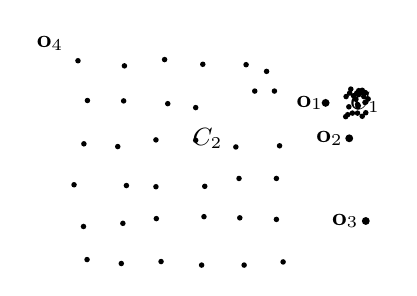
\begin{tikzpicture}[thick,scale=0.5, every node/.style={scale=5}]
			\fill (0.14, 0.02)  circle (0.7mm) (0.05, 0.86)  circle (0.7mm) (-0.19, 1.92)  circle (0.7mm) (0.06, 2.96)  circle (0.7mm) (0.15, 4.06)  circle (0.7mm) (-0.09, 5.07)  circle (0.7mm) (1.01, -0.08)  circle (0.7mm) (1.05, 0.94)  circle (0.7mm) (1.14, 1.9)  circle (0.7mm) (0.92, 2.89)  circle (0.7mm) (1.07, 4.05)  circle (0.7mm) (1.09, 4.94)  circle (0.7mm) (2.02, -0.03)  circle (0.7mm) (1.9, 1.06)  circle (0.7mm) (1.89, 1.87)  circle (0.7mm) (1.89, 3.06)  circle (0.7mm) (2.19, 3.98)  circle (0.7mm) (2.11, 5.1)  circle (0.7mm) (3.05, -0.12)  circle (0.7mm) (3.11, 1.11)  circle (0.7mm) (3.13, 1.88)  circle (0.7mm) (2.9, 3.05)  circle (0.7mm) (2.9, 3.88)  circle (0.7mm) (3.08, 4.98)  circle (0.7mm) (4.13, -0.12)  circle (0.7mm) (4.02, 1.08)  circle (0.7mm) (4.0, 2.08)  circle (0.7mm) (3.92, 2.88)  circle (0.7mm) (4.4, 4.3)  circle (0.7mm) (4.18, 4.97)  circle (0.7mm) (5.12, -0.04)  circle (0.7mm) (4.95, 1.04)  circle (0.7mm) (4.95, 2.08)  circle (0.7mm) (5.03, 2.91)  circle (0.7mm) (4.9, 4.3)  circle (0.7mm) (4.7, 4.8)  circle (0.7mm);

			% cluster
			\fill (7.22, 4.02)  circle (0.7mm) (7.01, 3.74)  circle (0.7mm) (7.17, 4.16)  circle (0.7mm) (7.04, 4.31)  circle (0.7mm) (7.28, 4.1)  circle (0.7mm) (7.22, 3.75)  circle (0.7mm) (6.99, 4.25)  circle (0.7mm) (7.13, 3.66)  circle (0.7mm) (7.03, 3.93)  circle (0.7mm) (6.84, 4.35)  circle (0.7mm) (6.72, 4.16)  circle (0.7mm) (7.14, 4.27)  circle (0.7mm) (6.88, 3.74)  circle (0.7mm) (7.04, 4.21)  circle (0.7mm) (6.79, 3.9)  circle (0.7mm) (7.01, 3.96)  circle (0.7mm) (7.13, 4.32)  circle (0.7mm) (6.71, 3.65)  circle (0.7mm) (6.76, 3.7)  circle (0.7mm) (7.21, 4.26)  circle (0.7mm) (7.02, 3.9)  circle (0.7mm) (7.2, 4.01)  circle (0.7mm) (6.91, 4.18)  circle (0.7mm) (6.81, 4.25)  circle (0.7mm) (6.97, 4.09)  circle (0.7mm);

			% outlier O3
			\fill (7.22, 1)  circle (1mm);
			\node[scale = 0.2] at (6.7, 1) {\small $\textbf{o}_3$};

			% O1
			\fill (6.2, 4)  circle (1mm);
			\node[scale = 0.2] at (5.8, 4) {\small $\textbf{o}_1$};

			% O2
			\fill (6.8, 3.1)  circle (1mm);
			\node[scale = 0.2] at (6.3, 3.1) {\small $\textbf{o}_2$};
			\node[scale = 0.2] at (7.2, 4) {\small $C_1$};
			\node[scale = 0.2] at (3.2, 3.1) {\small $C_2$};
			\node[scale = 0.2] at (-0.8, 5.5) {\small $\textbf{o}_4$};
		\end{tikzpicture}};
\end{frame}


\begin{frame}{Density-Based Outlier Detection: Measure Relative Density}
	\begin{itemize}
		\item Use the \textbf{relative density} of an object against its neighbors \\
		      as the indicator of the degree of the object being an outlier.
		\item \textbf{{\color{airforceblue}$k$-distance} of an object $\mathbf{o}$:} $d_k(\mathbf{o})$.

		      Distance between $\mathbf{o}$ and its $k$-nearest neighbors.
		\item Distance $d(\mathbf{o}, \mathbf{p})$ between $\mathbf{o}$ and its $k$-nearest neighbour $p$.
		      \begin{itemize}
			      \item At least $k$-objects $\textbf{o}' \in \mathbf{D} - \{\mathbf{o}\}$
			            such that $d(\mathbf{o}, \mathbf{o}') \leq d(\mathbf{o}, \mathbf{p})$.
			      \item At most $k-1$ objects $\mathbf{o}'' \in \mathbf{D} - \{\mathbf{o}\}$
			            such that $d(\mathbf{o}, \mathbf{o}'') > d(\mathbf{o}, \mathbf{p})$.
		      \end{itemize}
		\item $k$-distance neighborhood of $\mathbf{o}$:
		      \begin{itemize}
			      \item $N_k(\mathbf{o}) = \{\mathbf{o}' \; \vert \; \mathbf{o}' \in \mathbf{D}, d(\mathbf{o}, \mathbf{o}') \leq d_k(\mathbf{o})\}$.
			      \item $N_k(\mathbf{o})$ could be bigger than $k$ \\
			            since multiple objects may have identical distance to $\mathbf{o}$.
		      \end{itemize}
		\item Measure local distance by using the \textit{average distance} from objects in $N_k(\mathbf{o})$.
		\item \textbf{Problem:} If $\mathbf{o}$ has very close neighbors $\mathbf{o}'$, statistical fluctuations of the distance measure can be undesirable high. Overcome this problem with a \underline{reachability distance}.
	\end{itemize}
\end{frame}


\begin{frame}{Density-Based Outlier Detection: Reachability Distance}
	\begin{itemize}
		\item \textbf{\color{airforceblue}Reachability distance from $\mathbf{o'}$ to $\mathbf{o}$:}
		      \begin{align*}
			      \text{reachdist}_k(\mathbf{o}' \leftarrow \mathbf{o}) = \max \{d_k(\mathbf{o}), d(\mathbf{o},\mathbf{o}')\},
		      \end{align*}

		      where $k$ is a user-specified parameter that adds a smoothing effect.
		\item $k$ specifies the minimum neighborhood to be examined to determine the local density of an object.
		\item \textbf{Reachability distance is not symmetric!}
		      \begin{align*}
			      \text{reachdist}_k(\mathbf{o}' \leftarrow \mathbf{o}) \neq \text{reachdist}_k(\mathbf{o} \leftarrow \mathbf{o}')
		      \end{align*}
		\item \textbf{Local reachability density of $\mathbf{o}$:}
		      \begin{align*}
			      \text{ldr}_k(\mathbf{o}) = \frac{||N_k(\mathbf{o})||}{\sum_{\mathbf{o'} \in N_k(\mathbf{o})} \text{reachdist}_k(\mathbf{o'} \leftarrow \mathbf{o})}.
		      \end{align*}
	\end{itemize}
\end{frame}


\begin{frame}{Density-Based Outlier Detection: Local Outlier Factor (LOF)}
	\begin{itemize}
		\item LOF is the average of the ratio of the local reachability density of $\mathbf{o}$ and \\
		      those of $\mathbf{o}$'s $k$-nearest neighbors.
		\item The lower $\text{ldr}$ and the higher $\text{ldr}$ of the $k$-nearest neighbors of $\mathbf{o}$,\\
		      then the higher the LOF value.
		\item LOF of $\mathbf{o}$ is defined as:
		      \begin{align*}
			      \text{LOF}_k(\mathbf{o}) = \frac{\sum_{\mathbf{o'} \in N_k(\mathbf{o})} \frac{\text{lrd}_k(\mathbf{o'})}{\text{lrd}_k(\mathbf{o})}}{||N_k(\mathbf{o})||} =
			      \sum_{\mathbf{o'} \in N_k(\mathbf{o})} \text{lrd}_k(\mathbf{o'}) \cdot \sum_{\mathbf{o'} \in N_k(\mathbf{o})} \text{reachdist}_k(\mathbf{o'} \leftarrow \mathbf{o}).
		      \end{align*}
		\item This captures a local outlier whose local density is relatively low comparing to the local densities of its $k$-NN.

	\end{itemize}

\end{frame}

\section{Summary}

\begin{frame}{Summary}
	\centering
	\begin{itemize}
		\item \textbf{Data attribute types:}\\
		      Nominal, binary, ordinal, interval-scaled or ratio-scaled.
		\item \textbf{Many types of data sets:}\\
		      E.g. numerical, text, graph, web, image.
		\item \textbf{Gain insight into the data by:}
		      \begin{itemize}
			      \item Basic statistical data description: \emph{Central tendency, dispersion and graphical display.}
			      \item Data visualization: \emph{Map data onto graphical primitives.}
			      \item Measure data similarity.
		      \end{itemize}
		\item \textbf{Above steps are the beginning of data preprocessing.}
		\item \textbf{Many methods have been developed but still an active area of research.}
	\end{itemize}
\end{frame}

\begin{frame}[c]
	\begin{center}
		{\bf Any questions about this chapter?}\\[0.5cm]
		Ask them now or ask them later in our forum: \\\bigskip
		StudOn Forum \\
		\faLink\ \url{https://www.studon.fau.de/frm5045379.html} \smallskip

	\end{center}
\end{frame}

\appendix
\section{Appendix}

\begin{frame}{Maximum Likelihood Estimation}
	\begin{itemize}
		\item \textbf{Example:} Assume a normal distribution $\mathcal{N}(\mu, \sigma)$ with probability density function
		      \begin{align*}
			      f(x)=\frac{1}{\sqrt{2\pi \sigma^2}} {\rm e}^{-\frac{(x-\mu)^2}{2\sigma^2}}
		      \end{align*}
		\item Likelihood function of the normal distribution for a dataset $X=\{x_1, \dots, x_n\}$, therefore, is as follows:
		      \vspace{-0.8em}
		      \begin{equation*}
			      \mathcal{L}(\mu, \sigma|x_1, \dots, x_n) = \prod\nolimits_{i=1}^n \frac{1}{\sqrt{2\pi \sigma^2}} {\rm e}^{-\frac{(x_i-\mu)^2}{2\sigma^2}}
		      \end{equation*}
		\item General procedure:
		      \begin{enumerate}
			      \item Generate two derivatives, with respect to $\mu$ and $\sigma$, respectively.
			      \item Solve each equation by setting them equal to zero.
		      \end{enumerate}
		\item Instead of taking the derivative directly, we take the log of the likelihood function as this makes it easier to take derivatives.
	\end{itemize}
\end{frame}

\begin{frame}{Maximum Likelihood Estimation: Log-Transform Equation}
	\begin{columns}
		\begin{column}{0.6\textwidth}
			\vspace*{-2em}
			\begin{align*}
				 & \ln{\mathcal{L}(\mu, \sigma|x_1, \dots, x_n)}= \ln{\bigg(\eqmark{faured}{\textstyle\prod\nolimits_{i=1}^n}{e1} \frac{1}{\sqrt{2\pi \sigma^2}} {\rm e}^{-\frac{(x_i-\mu)^2}{2\sigma^2}}\bigg)}      \\
				 & =\textstyle\sum\nolimits_{i=1}^n \ln{\bigg(\eqmark{faured}{\frac{1}{\sqrt{2\pi \sigma^2}} {\rm e}^{-\frac{(x_i-\mu)^2}{2\sigma^2}}}{e2}\bigg)}                                                     \\
				 & =\textstyle\sum\nolimits_{i=1}^n \bigg(\ln{\bigg(\eqmark{faured}{\frac{1}{\sqrt{2\pi \sigma^2}}}{e3}\bigg)} + \ln{\bigg(\eqmark{faured}{{\rm e}^{-\frac{(x_i-\mu)^2}{2\sigma^2}}}{e4}\bigg)}\bigg) \\
				 & =\textstyle\sum\nolimits_{i=1}^n \left(\ln{\left((2\pi\sigma^2)^{-\frac{1}{2}} \right)} - \frac{(x_i-\mu)^2}{2\sigma^2} \ln{{\rm e}}\right)
			\end{align*}

			\begin{tikzpicture}[remember picture,overlay]
				\node[below=-1em of e1] (m1) {\color{faured}\small1.};
				\node[below=-1em of e2] (m2) {\color{faured}\small2.};
				\node[below=-1em of e3] (m2) {\color{faured}\small3.a};
				\node[below=-1em of e4] (m2) {\color{faured}\small3.b};
			\end{tikzpicture}

		\end{column}

		\begin{column}{0.4\textwidth}
			\begin{enumerate}
				{
				\setbeamercolor{enumerate item}{fg=faured}
				\item Log transforms multiplicatoin into addition.
				\item Transform each element in log, that is convert multiplication to addition.
				\item Convert one {\color{faured}(a)} over square root and {\color{faured}(b)} exponent of euler.

				      Recall:
				      \vspace*{-1em}
				      \begin{align*}
					      x^{-v}      & = \frac{1}{x^v}  \\
					      \sqrt[v]{x} & =x^{\frac{1}{v}} \\
					      \ln{x^v}    & =v\ln{x}
				      \end{align*}
				      }
			\end{enumerate}
		\end{column}
	\end{columns}
\end{frame}

\begin{frame}{Maximum Likelihood Estimation: Log-Transform Equation}
	\vspace*{-2em}
	\begin{columns}
		\begin{column}{0.5\textwidth}
			\begin{align*}
				 & =\textstyle\sum\nolimits_{i=1}^n \Big(\ln{\Big(\eqmark{faured}{(2\pi\sigma^2)^{-\frac{1}{2}}}{e5} \Big)} - \frac{(x_i-\mu)^2}{2\sigma^2} \eqmark{faured}{\ln{{\rm e}}}{e6}\Big) \\
				 & =\textstyle\sum\nolimits_{i=1}^n \Big(-\frac{1}{2}\ln{\eqmark{faured}{2\pi\sigma^2}{e7}}-\eqmark{faured}{\frac{(x_i-\mu)^2}{2\sigma^2}}{e8}\Big)                                \\
				 & =\textstyle\sum\nolimits_{i=1}^n \Big(-\frac{1}{2}\ln{2\pi}-\frac{1}{2}\eqmark{faured}{\ln{\sigma^2}}{e9}-\frac{(x_i-\mu)^2}{2\sigma^2}\Big)                                    \\
				 & =\textstyle\sum\nolimits_{i=1}^n \Big(-\frac{1}{2}\ln{2\pi}-\eqmark{faured}{\textstyle\frac{1}{2}2}{e10}\ln{\sigma}-\frac{(x_i-\mu)^2}{2\sigma^2}\Big)                          \\
				 & =\textstyle\sum\nolimits_{i=1}^n \left(-\frac{1}{2}\ln{2\pi}-\ln{\sigma}-\frac{(x_i-\mu)^2}{2\sigma^2}\right)\tikzmark{e11}
			\end{align*}
			\begin{tikzpicture}[remember picture,overlay]
				\node[below=-1em of e5] (m1) {\color{faured}\small4.a};
				\node[below=-1em of e6] (m2) {\color{faured}\small4.b};
				\node[below=-1em of e7] (m3) {\color{faured}\small5.a};
				\node[below=-1em of e8] (m4) {\color{faured}\small5.b};
				\node[below=-1em of e9] (m5) {\color{faured}\small6.};
				\node[below=-1em of e10] (m6) {\color{faured}\small7.};
			\end{tikzpicture}
		\end{column}

		\begin{column}{0.5\textwidth}
			\begin{enumerate}
				{
				\setbeamercolor{enumerate item}{fg=faured}
				\setcounter{enumi}{3}
				\item Convert {\color{faured}(a)} exponent into multiplication and {\color{faured}(b)} remove $\ln{\rm e}$.

				      Recall:
				      \vspace*{-1em}
				      \begin{align*}
					      \ln{\rm e}=1
				      \end{align*}
				\item {\color{faured}(a)} Transform multiplication to addition. {\color{faured}(b)} Nothing to do to last term.
				\item Convert exponent.
				\item Simplify equation.
				      }
			\end{enumerate}

			\vspace*{1em}
			\textbf{We can now take the derivative w.\,r.\,t. $\mu$ and $\sigma$ of:}
			\vspace*{-1em}
			\begin{align*}
				 & \ln{(\mathcal{L}(\mu, \sigma|x_1, \dots, x_n))}                                                        \\
				 & \tikzmark{e12}=-\textstyle\frac{n}{2}\ln{2\pi}-n\ln{\sigma}-\sum_{i=1}^n \frac{(x_i-\mu)^2}{2\sigma^2}
			\end{align*}
			\begin{tikzpicture}[remember picture,overlay]
				\draw[faured,thick,->] ([yshift=1.2mm,xshift=1mm]e11) to[out=5,in=180] ([yshift=1mm,xshift=-1mm]e12) node [above right=0.1em and 3.3em of e11] (m7) {\small{\color{faured}7.}};
			\end{tikzpicture}
		\end{column}
	\end{columns}
\end{frame}

\begin{frame}{Maximum Likelihood Estimation: Take Derivative w.\,r.\,t. $\mu$}
	\vspace*{-2em}
	\begin{columns}
		\begin{column}{0.5\textwidth}
			\begin{align*}
				 & \textstyle\frac{\partial}{\partial \mu}\ln{(\mathcal{L}(\mu, \sigma|x_1, \dots, x_n))}                                                                                                                                                                                            \\
				 & =\eqmark{fauorange}{\textstyle\frac{\partial}{\partial \mu}(-\frac{n}{2}\ln{2\pi})}{e1}-\eqmark{fauorange}{\textstyle\frac{\partial}{\partial \mu}(n\ln{\sigma}}{e2})-\sum_{i=1}^{n} \eqmark{fauorange}{\textstyle\frac{\partial}{\partial \mu}\frac{(x_i-\mu)^2}{2\sigma^2}}{e3} \\
				 & =\eqmark{fauorange}{\textstyle\sum_{i=1}^n \frac{-2(x_i-\mu)(-1)}{2\sigma^2}}{e4}                                                                                                                                                                                                 \\
				 & =\textstyle\sum_{i=1}^n\frac{2(x_i-\mu)}{2\sigma^2}                                                                                                                                                                                                                               \\
				 & = \textstyle\sum_{i=1}^n \frac{x_i-\mu}{\sigma^2}                                                                                                                                                                                                                                 \\
				 & = \frac{1}{\sigma^2} \sum_{i=1}^n (x_i -\mu)
			\end{align*}
			\begin{tikzpicture}[remember picture,overlay]
				\node[below=-1em of e1] (m1) {\color{fauorange}\small1.};
				\node[below=-1em of e2] (m2) {\color{fauorange}\small1.};
				\node[below=-1em of e3] (m2) {\color{fauorange}\small2.};
				\node[below=-1em of e4] (m2) {\color{fauorange}\small3.};
			\end{tikzpicture}
		\end{column}
		\begin{column}{0.5\textwidth}
			\begin{enumerate}
				{
				\setbeamercolor{enumerate item}{fg=fauorange}
				\item Derivative of this component can be treated as a constant as it does not contain $\mu$, therefore it equals to zero.
				\item Apply chain rule.
				\item Simplify equation.
				      }
			\end{enumerate}
			\vspace*{1em}
			{
				\footnotesize
				Recall:
				\vspace*{-1em}
				\begin{align*}
					\text{Linearity: } (f+g)'                                        & = f' + g'                                                                       \\
					\text{Product Rule: } (fg)'                                      & = f'g + fg'                                                                     \\
					\text{Quotient: } \left(\textstyle\frac{f}{g}\right)'            & =\textstyle\frac{f'g-fg'}{g^2}                                                  \\
					\text{Chain Rule: } (f(g(x)))'                                   & =f'(g(x))g'(x)                                                                  \\
					\text{also denoted as: } \textstyle\frac{\partial f}{\partial x} & =\textstyle\frac{\partial f}{\partial g}\textstyle\frac{\partial g}{\partial x}
				\end{align*}
			}
		\end{column}
	\end{columns}
\end{frame}

\begin{frame}{Maximum Likelihood Estimation: Take Derivative w.\,r.\,t. $\sigma$}
	\begin{columns}
		\begin{column}{0.5\textwidth}
			\vspace*{-2em}
			\begin{align*}
				 & \textstyle\frac{\partial}{\partial \sigma}\ln{(\mathcal{L}(\mu, \sigma|x_1, \dots, x_n))}                                                                                                                                                                                            \\
				 & =\eqmark{faucyan}{\textstyle\frac{\partial}{\partial \sigma}(-\frac{n}{2}\ln{2\pi})}{e1}-\eqmark{faucyan}{\textstyle\frac{\partial}{\partial \sigma}(n\ln{\sigma}}{e2})-\sum_{i=1}^{n} \eqmark{faucyan}{\textstyle\frac{\partial}{\partial \sigma}\frac{(x_i-\mu)^2}{2\sigma^2}}{e3} \\
				 & =-\textstyle\frac{n}{\sigma}\eqmark{faucyan}{-\textstyle\sum_{i-1}^n \frac{(x_i-\mu)^2}{2}(-2)\sigma^{-3}}{e4}                                                                                                                                                                       \\
				% &=-\textstyle\frac{n}{\sigma}+\sum_{i=1}^n \frac{(x_i-\mu)^2}{2}(2)\sigma^{-3}\\
				 & =-\textstyle\frac{n}{\sigma}+\sum_{i=1}^n (x_i-\mu)^2\eqmark{faucyan}{\sigma^{-3}}{e5}                                                                                                                                                                                               \\
				 & =\eqmark{faucyan}{-\textstyle\frac{n}{\sigma}+\sum_{i=1}^n \frac{(x_i-\mu)^2}{\sigma^3}}{e6}                                                                                                                                                                                         \\
				 & =-\textstyle\frac{n}{\sigma}+\frac{1}{\sigma^3}\sum_{i=1}^n (x_i-\mu)^2
			\end{align*}
			\begin{tikzpicture}[remember picture,overlay]
				\node[below=-1em of e1] (m1) {\color{faucyan}\small1.};
				\node[below=-1em of e2] (m2) {\color{faucyan}\small2.};
				\node[below=-1em of e3] (m2) {\color{faucyan}\small3.};
				\node[below=-1em of e4] (m2) {\color{faucyan}\small4.};
				\node[below=-1em of e5] (m2) {\color{faucyan}\small5.};
				\node[below=-1em of e6] (m2) {\color{faucyan}\small6.};
			\end{tikzpicture}
		\end{column}
		\begin{column}{0.5\textwidth}
			\begin{enumerate}
				{
				\setbeamercolor{enumerate item}{fg=faucyan}
				\item Derivative of this component can be treated as a constant as it does not contain $\sigma$, therefore it equals to zero.
				\item Take derivative.
				\item Easier when expressed as $\frac{(x_i-\mu)^2}{2}\sigma^{-2}$. Then take derivative of $\sigma^{-2}$. Recall: $(x^a)'=ax^{a-1}$
				\item Two minuses cancel out (minus before sum and minus of $(-2)$). Additionally, simplify by cancel out $\frac{2}{2}$.
				\item Put back as denominator.
				\item Simplify equation.
				      }
			\end{enumerate}
		\end{column}
	\end{columns}
\end{frame}

\begin{frame}{Maximum Likelihood Estimation: Two Derivatives w.\,r.\,t. $\mu$ and $\sigma$}
	\vspace*{-1em}
	Derivatives are:
	\vspace*{-2em}
	\begin{align*}
		\textstyle\frac{\partial}{\partial \mu}\ln{(\mathcal{L}(\mu, \sigma|x_1, \dots, x_n))}    & = \frac{1}{\sigma^2} \sum_{i=1}^n (x_i -\mu)                            \\
		\textstyle\frac{\partial}{\partial \sigma}\ln{(\mathcal{L}(\mu, \sigma|x_1, \dots, x_n))} & =-\textstyle\frac{n}{\sigma}+\frac{1}{\sigma^3}\sum_{i=1}^n (x_i-\mu)^2
	\end{align*}

	\textbf{To find the estimates of $\mu$ and $\sigma$, solve these equations by equal them to zero\footnote{We want to find the value for with the log functions reaches their maximum. At this point, the slope of these functions equal to zero. Therefore, we equal these functions to zero.}:}

	\begin{itemize}
		\item For $\mu$: $0=\textstyle\frac{1}{\sigma^2} \sum_{i=1}^n (x_i -\mu) \stackrel{{\color{faured}\times \sigma^2}}{\Leftrightarrow} 0=\sum_{i=1}^n x_i-\mu \stackrel{{\color{faured}+n\mu}}{\Leftrightarrow} n\mu = \sum_{i=1}^n x_i \stackrel{{\color{faured}\times\frac{1}{n}}}{\Leftrightarrow} \underline{\underline{\mu=\frac{1}{n}\sum_{i=1}^n x_i}}$\\This equals to mean.
		\item For $\sigma$: $0=-\textstyle\frac{n}{\sigma}+\frac{1}{\sigma^3}\sum_{i=1}^n (x_i-\mu)^2 \stackrel{{\color{faured}\times \sigma}}{\Leftrightarrow} 0=-n+\frac{1}{\sigma^2}\sum_{i=1}^n (x_i-\mu)^2 \stackrel{{\color{faured}+n}}{\Leftrightarrow} n=\frac{1}{\sigma^2} \sum_{i=1}^n (x_i-\mu)^2$\\
		      $\stackrel{{\color{faured}\times \sigma^2}}{\Leftrightarrow} n\sigma^2 = \sum_{i=1}^n (x_i-\mu)^2 \stackrel{{\color{faured}\times \frac{1}{n}}}{\Leftrightarrow} \sigma^2 = \frac{1}{n}\sum_{i=1}^n (x_i-\mu)^2 \stackrel{{\color{faured}\sqrt{\vphantom{}}}}{\Leftrightarrow} \underline{\underline{\sigma=\sqrt{\frac{1}{n}\sum_{i=1}^n (x_i-\mu)^2}}}$\\This equals to standard deviation.
	\end{itemize}
\end{frame}

\end{document}
